%-----------------------------------------------
%  Engineer's & Master's Thesis Template
%  Copyleft by Artur M. Brodzki & Piotr Woźniak
%  Warsaw University of Technology, 2019-2022
%-----------------------------------------------

\documentclass[
    bindingoffset=5mm,  % Binding offset
    footnoteindent=3mm, % Footnote indent
    hyphenation=true    % Hyphenation turn on/off
]{src/wut-thesis}

\graphicspath{{tex/img/}} % Katalog z obrazkami.
\addbibresource{bibliografia.bib} % Plik .bib z bibliografią

%-------------------------------------------------------------
% Wybór wydziału:
%  \facultyeiti: Wydział Elektroniki i Technik Informacyjnych
%  \facultymeil: Wydział Mechaniczny Energetyki i Lotnictwa
% --
% Rodzaj pracy: \EngineerThesis, \MasterThesis
% --
% Wybór języka: \langpol, \langeng
%-------------------------------------------------------------
\facultyeiti    % Wydział Elektroniki i Technik Informacyjnych
\EngineerThesis % Praca inżynierska
\langpol % Praca w języku polskim

\begin{document}

%------------------
% Strona tytułowa
%------------------
\instytut{Informatyki}
\kierunek{Informatyka}
\specjalnosc{Sztuczna Inteligencja}
\title{
    Projekt inteligentnej bramy (Gateway) oraz narzędzia CLI do \\ semantycznej deduplikacji danych w systemach Cloud Storage
}
% Title in English for English theses
% In English theses, you may remove this command
\engtitle{
    Design of an intelligent gateway and a CLI tool \\
    for semantic data deduplication in cloud storage systems
}

\author{Kacper Górski}
\album{331379}
\promotor{dr. inż. Łukasz Lepak}
\date{\the\year}
\maketitle

%-------------------------------------
% Streszczenie po polsku dla \langpol
% English abstract if \langeng is set
%-------------------------------------
\cleardoublepage % Zaczynamy od nieparzystej strony
\abstract
Chmurowe magazyny obiektowe, takie jak Amazon S3, pozwalają na niemal nieograniczoną skalowalność przechowywania danych. W systemach, do których trafia duża liczba plików graficznych, np. w serwisach e-commerce, mediach społecznościowych czy archiwach zdjęć, model rozliczeniowy Pay-As-You-Go sprawia jednak, że utrzymywanie redundantnych danych generuje wysokie koszty. Ten sam obraz jest często przesyłany wielokrotnie w różnych rozdzielczościach, formatach (np. PNG i silnie skompresowany JPEG) lub z drobnymi artefaktami kompresji. Klasyczne podejście do weryfikacji tożsamości danych, oparte na funkcjach skrótu (takich jak MD5 czy SHA-256), okazuje się w takiej sytuacji niewystarczające. Ze względu na tzw. efekt lawinowy zmiana choćby jednego bajtu pliku daje zupełnie inny skrót, przez co obrazy niemal identyczne wizualnie nie są rozpoznawane jako duplikaty, a przestrzeń dyskowa jest marnowana.

W pracy przedstawiono koncepcję oraz implementację inteligentnej bramy deduplikacyjnej, która wykorzystuje modele sztucznej inteligencji do analizy semantycznej przesyłanych obrazów. Zamiast porównywać zawartość bajtową, system przekształca każdy obraz w wielowymiarowy wektor (ang. \emph{embedding}) za pomocą modelu SSCD, przeznaczonego do wykrywania kopii obrazów, a podobieństwo wektorów wyznacza miarą kosinusową (ang. \emph{cosine similarity}). Gdy zostanie wykryty obraz o wysokim stopniu podobieństwa do już przechowywanego, mechanizm porównuje jakość obu wersji na podstawie metryk bezreferencyjnych, m.in. BRISQUE oraz wariancji laplasjanu jako miary ostrości. Dzięki temu duplikaty gorszej jakości są odrzucane, a słabsze wersje obrazów mogą zostać zastąpione wersjami o lepszej jakości.

Zaimplementowana architektura hybrydowa składa się z autorskiego narzędzia CLI napisanego w języku Go, które pośredniczy w operacjach zapisu, oraz połączonego z nim lokalnego mikroserwisu w języku Python, w którym uruchomiony jest model wektorowy. Logika przetwarzania działa w środowisku lokalnym i jest bezpośrednio zintegrowana z usługami chmury AWS. W celu zwiększenia wydajności proces podzielono na dwa etapy. W pierwszym dokładne duplikaty są wykrywane z użyciem bazy klucz-wartość Amazon DynamoDB, co pozwala odrzucić powtarzające się pliki w czasie $O(1)$. W drugim nowe dane poddawane są właściwej analizie semantycznej. Reprezentacje wektorowe przechowywane są w bazie PostgreSQL z rozszerzeniem pgvector, umożliwiającym wydajne wyszukiwanie najbliższych sąsiadów, natomiast zdeduplikowane pliki trafiają do standardowych zasobników Amazon S3. Część badawcza pracy osadzona jest w metodyce FinOps i ma na celu określenie, przy jakiej skali i charakterystyce danych wdrożenie takiego mechanizmu przynosi wymierne korzyści finansowe.

\keywords Cloud Storage, Amazon S3, deduplikacja semantyczna, deduplikacja obrazów, embeddingi, SSCD, ocena jakości obrazu, Amazon DynamoDB, pgvector, FinOps
%----------------------------------------
% Streszczenie po angielsku dla \langpol
% Polish abstract if \langeng is set
%----------------------------------------
\clearpage
\secondabstract
Cloud object storage services such as Amazon S3 offer almost unlimited scalability. In systems that receive large numbers of image files, e.g. e-commerce platforms, social media or photo archives, the Pay-As-You-Go billing model makes storing redundant data expensive. The same image is often uploaded many times in different resolutions, formats (e.g. PNG and heavily compressed JPEG) or with minor compression artifacts. The classic approach to verifying data identity, based on hash functions such as MD5 or SHA-256, is not sufficient in this case. Because of the avalanche effect, changing even a single byte of a file produces a completely different hash, so visually near-identical images are not recognised as duplicates and storage space is wasted.

This thesis presents the design and implementation of an intelligent deduplication gateway that uses artificial intelligence models to perform semantic analysis of uploaded images. Instead of comparing raw bytes, the system converts each image into a high-dimensional vector (embedding) using the SSCD copy detection model and measures similarity between vectors with cosine similarity. When an image highly similar to an already stored one is detected, the mechanism compares the quality of both versions using no-reference metrics, including BRISQUE and the variance of the Laplacian as a sharpness measure. As a result, lower-quality duplicates are rejected and weaker versions of images can be replaced with better ones.

The implemented hybrid architecture consists of a custom CLI tool written in Go, which mediates write operations, and a connected local Python microservice that runs the embedding model. The processing logic runs locally and is directly integrated with AWS cloud services. To improve performance, the process is divided into two stages. First, exact duplicates are detected using the Amazon DynamoDB key-value database, which allows repeated files to be rejected in $O(1)$ time. Second, new data undergoes the actual semantic analysis. Vector representations are stored in PostgreSQL with the pgvector extension, which enables efficient nearest-neighbour search, while deduplicated files are stored in standard Amazon S3 buckets. The research part of the thesis follows the FinOps methodology and aims to determine at what scale and for which data characteristics deploying such a mechanism brings measurable financial benefits.
\secondkeywords Cloud Storage, Amazon S3, semantic deduplication, image deduplication, embeddings, SSCD, image quality assessment, Amazon DynamoDB, pgvector, FinOps

\pagestyle{plain}

%--------------
% Spis treści
%--------------
\cleardoublepage % Zaczynamy od nieparzystej strony
\tableofcontents

%------------
% Rozdziały
%------------
\cleardoublepage % Zaczynamy od nieparzystej strony
\pagestyle{headings}

\clearpage % Rozdziały zaczynamy od nowej strony.
\section{Praefatio}

% Akapit z cytatem
\lipsum[1] \cite{goossens93}

% Przykładowy obrazek
\begin{figure}[!h]
    % Wyrównanie obrazka, szerokość i plik
    % Zamiast width można też użyć height, etc.
    \centering 
\includegraphics[width=0.5\linewidth]{logopw.png}
    % Podpis umieszczamy pod obrazkiem
    % znacznik \caption służy również do wygenerowania numeru obrazka
    \caption{Tradycyjne godło Politechniki Warszawskiej}
    % \label pozwala odwołać się do obrazka w innych miejscach za pomocą \ref
    % odwołanie \ref renderuje się jako numer obrazka,
    % dlatego zawsze najpierw używaj \caption a potem \label
    \label{fig:tradycyjne-logo-pw}
\end{figure}

% \ref wyrenderuje się jako 'Reference to image 1.1'
\lipsum[2] Reference to image \ref{fig:tradycyjne-logo-pw}.

% Lista punktowana
% Parametr label ustawia symbol punktora
\begin{itemize}
    \item Item 1:
    \begin{itemize}[label=---]
        \item item 1.1;
        \item item 1.2;
    \end{itemize}
    \item Item 2;
    \item Item 3.
\end{itemize}

\lipsum[3]

% Lista numerowana w formacie 1.a).ii
% Tutaj również można stosować \label
\begin{enumerate}
    \item Item 1:
    \begin{enumerate}
        \item item 1.1;
        \item item 1.2:
        \begin{enumerate}
            \item item 1.2.1;
            \item item 1.2.2;
        \end{enumerate}
        \item item 1.3;
    \end{enumerate}
    \item Item 2;
    \item Item 3.
\end{enumerate}

% Przypis dolny \footnote
\lipsum[4] Lorem ipsum dolor sit amet\footnote{Lorem ipsum dolor sit amet, consectetur adipiscing elit, sed do eiusmod tempor incididunt ut labore et dolore magna aliqua. Ut enim ad minim veniam, quis nostrud exercitation ullamco laboris nisi ut aliquip ex ea commodo consequat.}, consectetur adipiscing elit.

% Przykładowa tabela: wyśrodkowana i renderowana
% w miejscu wstawienia: !h = !h[ere]
% Domyślnie tabele trafiają na górę strony
\begin{table}[!h] \centering
    % Podpis tabeli umieszczamy od góry
    \caption{Przykładowa tabela.}
    \label{tab:tabela1}

    % Tabela z trzema kolumnami:
    % dwie wyrównanie do środka [c], a ostatnia do prawej [r]
    % szerokość kolumn automatyczna (równa szerokości tekstu)
    \begin{tabular}{| c | c | r |} \hline
        Kolumna 1       & Kolumna 2 & Liczba \\ \hline\hline
        cell1           & cell2     & 60     \\ \hline
        cell4           & cell5     & 43     \\ \hline
        cell7           & cell8     & 20,45  \\ \hline
        % Komórka o szerokości dwóch kolumn, wyrównana do prawej
        % Przypisy dolne w tabelach wstawiamy przez \tablefootnote
        \multicolumn{2}{|r|}{Suma\tablefootnote{Table footnote.}} & 123,45 \\ \hline
    \end{tabular}

\end{table}

Lorem ipsum dolor sit amet.
         % Wygodnie jest trzymać każdy rozdział w osobnym pliku.
\clearpage % Rozdziały zaczynamy od nowej strony.
\section{Analiza dziedziny i przegląd technologii}


Przed rozpoczęciem pracy należy wprowadzić koncepcje i technologie wykorzystane do budowy inteligentnej bramy deduplikacyjnej. Opisano czym właściwie jest chmura publiczna Amazon Web Services, specyfikę obiektowych magazynów danych oraz baz dokumentowych na podstawie usług Amazon S3 oraz Amazon DynamoDB. Skonfrontowano także tradycyjne, oparte na funkcjach skrótu metody weryfikacji powielonych danych z podejściem semantycznym, które bazuje na wektorowych modelach wizyjnych.
% =========== Czym wogole jest AWS ====================

\subsection{Platforma Amazon Web Services}

\begin{figure}[!h]
    \centering
    
\includegraphics[width=0.12\linewidth]{Amazon_Web_Services_Logo.png}
    \caption{Logo Amazon Web Services. Źródło: Wikimedia Commons \cite{commons_wikimedia_aws}.}
    \label{fig:aws-icon}
\end{figure}

Amazon Web Services (AWS) stanowi zbiór usług chmurowych udostępnianych przez firmę Amazon, obejmujący ponad dwieście produktów przeznaczonych do przechowywania, przetwarzania oraz analizy danych \cite{aws_overview}. Zasoby przydzielane są na żądanie, a opłaty naliczane według rzeczywistego zużycia -- bez obowiązku wcześniejszej rezerwacji infrastruktury \cite{aws_pricing}. Platforma działa w ramach regionów geograficznych. Każdy z nich obejmuje co najmniej dwie odseparowane strefy dostępności, połączone siecią o niskich opóźnieniach \cite{aws_global_infrastructure}.

W opracowywanej bramie deduplikacyjnej wykorzystano trzy usługi tej platformy. Amazon S3 służy jako magazyn obiektowy dla plików graficznych wraz z metadanymi. Amazon DynamoDB pełni funkcję indeksu dokładnych duplikatów, przeszukiwanego za pomocą operacji \texttt{Query} i \texttt{GetItem}~\cite{aws_query_api,awsGetItem}. Komponent obliczeniowy pracuje lokalnie, lecz współpracuje z usługami AWS za pośrednictwem oficjalnych SDK \cite{aws_sdk_docs} -- dzięki temu całe rozwiązanie można przenieść do chmury bez modyfikacji logiki biznesowej.

Rozliczenia w AWS opierają się na modelu Pay-As-You-Go: koszt usługi zależy od zajętej przestrzeni dyskowej, liczby wykonanych operacji API oraz objętości transferu danych \cite{aws_pricing, aws_pricing_how_it_works}. Zależność ta stanowi bezpośrednią motywację dla deduplikacji -- odrzucenie każdej kopii obrazu eliminuje koszt przechowywania i zapisu jej danych binarnych, nie wyklucza jednak osobnego zapisu metadanych.

% =========== Amazon Simple Storage Service ===========


\subsection{Przechowywanie danych w chmurze -- Amazon S3}

\begin{figure}[!h]
    \centering
    
\includegraphics[width=0.12\linewidth]{Arch_Amazon-Simple-Storage-Service_64@5x.png}
    \caption{Ikona usługi Amazon S3. Źródło: AWS Architecture Icons \cite{aws_architecture_icons}.}
    \label{fig:aws-s3-icon}
\end{figure}

Amazon Simple Storage Service (S3) to usługa typu \textit{Object Storage}, przeznaczona do przechowywania dużych zbiorów danych w postaci binarnej (BLOB) \cite{aws_s3_service, aws_s3_welcome_doc}. W odróżnieniu od tradycyjnych systemów plików o strukturze drzewiastej, magazyny obiektowe przechowują dane w płaskiej przestrzeni, a widoczne w interfejsie użytkownika foldery są jedynie logicznym grupowaniem. Takie podejście ułatwia rozpraszanie danych w chmurze, zapewniając wysoką dostępność i łatwość skalowania.


\subsubsection{Architektura danych: Zasobniki i Obiekty}


Struktura S3 opiera się na dwóch podstawowych pojęciach \cite{aws_s3_service, aws_s3_welcome_doc}:
\begin{itemize}
    \item \textbf{Zasobniki (ang. \textit{Buckets})} -- Kontenery najwyższego poziomu. Domyślnie nazwa każdego zasobnika musi być unikalna w skali globalnej (od 2026 roku można też tworzyć zasobniki we własnej, regionalnej przestrzeni nazw konta \cite{aws_s3_namespaces}), choć fizycznie przypisuje się go do konkretnego regionu AWS (np. \texttt{us-east-1} znajdujący się w Północnej Wirginii w USA). Na poziomie zasobnika konfiguruje się m.in. polityki dostępu IAM oraz reguły retencji danych.
    \item \textbf{Obiekty (ang. \textit{Objects})} -- Właściwe pliki przechowywane w zasobnikach. Na obiekt składają się dane binarne (do 50 TB na pojedynczy plik \cite{aws_s3_50tb}), metadane oraz unikalny klucz (ang. \textit{Key}), który pełni rolę identyfikatora w ramach zasobnika.
\end{itemize}


\subsubsection{Zarządzanie metadanymi}


Metadane w S3, zapisywane jako pary klucz-wartość, dostarczają dodatkowych informacji o obiektach i dzielą się na dwie grupy \cite{aws_s3_service, aws_s3_welcome_doc}:
\begin{itemize}
    \item \textbf{Systemowe} -- Generowane przez AWS (np. rozmiar pliku, data modyfikacji, znacznik \textit{ETag}). W przypadku obiektów przesłanych pojedynczym żądaniem \texttt{PUT}, bez szyfrowania kluczem SSE-KMS lub SSE-C, \textit{ETag} jest skrótem MD5 zawartości pliku \cite{aws_s3_integrity}.
    \item \textbf{Użytkownika} -- Niestandardowe parametry nadawane przez aplikację podczas tworzenia obiektu, przesyłane w nagłówkach HTTP z prefiksem \texttt{x-amz-meta-}.
\end{itemize}


W bramie deduplikacyjnej opis pliku przechowywany jest jako osobny obiekt JSON. Otrzymuje on klucz \texttt{metadata/\allowbreak<file\_name>.json}, a dane obrazu zapisywane są niezależnie pod \texttt{payloads/\allowbreak<file\_name>}. Opis JSON należy odróżnić od metadanych użytkownika w nagłówkach \texttt{x-amz-meta-}, które są atrybutami dołączonymi do obiektu S3~\cite{aws_s3_object_metadata}. JSON przesyłany jest jako treść obiektu metodą \texttt{PutObject}, która zapisuje dane pod wskazanym kluczem w zasobniku~\cite{aws_s3_put_object}. Aktualizacja tego opisu nie wymaga kopiowania obrazu na niego samego. Kolejność zapisu metadanych i obrazu przedstawiono w podrozdziale~\ref{subsec:similarity-grpc-pipeline}.


\subsubsection{Model rozliczeniowy i optymalizacja kosztów (FinOps)}


Użycie usług takich jak S3 wiąże się z modelem płatności \textit{Pay-As-You-Go}, w którym koszty zależą od faktycznego zużycia zasobów. Składają się na nie trzy główne elementy \cite{aws_s3_service, aws_s3_welcome_doc}:
\begin{enumerate}
    \item \textbf{Wolumen danych} -- Miesięczna opłata za fizycznie zajętą przestrzeń.
    \item \textbf{Transfer (Data Egress)} -- Koszt przesyłania danych poza infrastrukturę AWS.
    \item \textbf{Operacje API} -- Opłaty za żądania sieciowe, przy czym operacje modyfikujące stan (\texttt{PUT}, \texttt{COPY}, \texttt{POST}) są znacznie droższe niż operacje odczytu (\texttt{GET}).
\end{enumerate}


Wdrożenie inteligentnej bramy deduplikacyjnej ma na celu redukcję tych wskaźników. Odrzucanie powielonych obrazów ogranicza zapis danych binarnych w S3, nie eliminuje jednak wszystkich operacji zapisu. Po decyzji deduplikacji nadal zapisywany jest osobny obiekt JSON z metadanymi; służy do tego \texttt{PutObject}, czyli operacja dodania obiektu do zasobnika~\cite{aws_s3_put_object}. W analizie kosztów należy więc uwzględnić zarówno pominięty zapis obrazu, jak i zapis JSON-a.


% =========== Amazon DynamoDB ===========

\subsection{Amazon DynamoDB jako szybki indeks duplikatów}

\begin{figure}[!h]
    \centering
    
\includegraphics[width=0.12\linewidth]{Arch_Amazon-DynamoDB_64@5x.png}
    \caption{Ikona usługi Amazon DynamoDB. Źródło: AWS Architecture Icons \cite{aws_architecture_icons}.}
    \label{fig:aws-dynamodb-icon}
\end{figure}

Amazon DynamoDB to zarządzana, rozproszona baza danych NoSQL typu klucz-wartość, zapewniająca stałą, niską latencję dostępu przy dużych wolumenach zapisu i odczytu \cite{aws_dynamodb_docs, aws_dynamodb_keyvalue}. Rekord identyfikowany jest przez klucz główny (ang. \textit{primary key}), składający się z klucza partycji (ang. \textit{partition key}) albo pary: klucz partycji i klucz sortowania (ang. \textit{sort key}). Przy kluczu złożonym dopiero ta para jednoznacznie identyfikuje rekord~\cite{aws_dynamodb_components}.

W projektowanej bramie deduplikacyjnej DynamoDB pełni funkcję indeksu dokładnych duplikatów. Do wstępnego wyszukiwania wykorzystywany jest skrót SHA-256 pierwszego fragmentu wyznaczonego przez CDC, a nie skróty wszystkich fragmentów pliku. Zastosowana biblioteka \texttt{restic/chunker} wyznacza granice na podstawie kroczącego odcisku Rabina~\cite{restic2026chunker}. Skróty \(c\) i \(h\), oznaczające odpowiednio skrót początkowego fragmentu i całego pliku, tworzą rekord \texttt{PK = CHUNK\#<c>}, \texttt{SK = FULL\#<h>}. Osobny rekord \texttt{PK = FILE\#<file\_name>}, \texttt{SK = META} przechowuje metadane potrzebne do zapisu i podmiany obiektu; nie stanowi dodatkowego etapu detekcji duplikatu.

Wyszukiwanie rozpoczyna się od \texttt{Query} dla klucza partycji \texttt{CHUNK\#<c>} z parametrem \texttt{Limit = 1}. Operacja ta pozwala odczytać elementy o wskazanej wartości klucza partycji~\cite{aws_query_api}. Dopiero po trafieniu obliczany jest pełny skrót \(h\) i wykonywane \texttt{GetItem} dla pary \texttt{CHUNK\#<c>}/\texttt{FULL\#<h>}; odczyt pojedynczego elementu wymaga wówczas obu składowych klucza~\cite{awsGetItem}. Jeżeli pierwszy odczyt nie zwróci kandydata, pełny skrót jest pomijany na etapie wyszukiwania, ale zostaje uzupełniony przed zapisem zaakceptowanego obrazu. Szczegóły przedstawiono w podrozdziałach~\ref{subsubsec:potok-cdc} i~\ref{subsubsec:potok-full-hash}.

Dzięki temu dokładne duplikaty są odrzucane przed uruchomieniem modelu wektorowego, co ogranicza liczbę wywołań modelu, opóźnienie odpowiedzi oraz koszty obliczeniowe systemu.


% =========== Classing Dedup using MD5 & SHA256 ===========


\subsection{Klasyczna deduplikacja oparta na funkcjach skrótu}


W tradycyjnych systemach redundancję danych eliminuje się z użyciem kryptograficznych funkcji skrótu (ang. \textit{hashing algorithms}). Funkcja taka przetwarza strumień wejściowy, generując sygnaturę o stałej długości, która w praktyce służy jako unikalny identyfikator pliku. Zakłada się przy tym, że prawdopodobieństwo kolizji (wygenerowania tego samego skrótu dla dwóch różnych plików) jest pomijalnie małe.


Weryfikacja polega na wyliczeniu skrótu $H_{new}$ dla nowego pliku $F_{new}$ i wyszukaniu go w indeksie systemu. Odczyt rekordu po kluczu należy odróżnić od kosztu obliczenia skrótu: \texttt{GetItem} odczytuje wskazany element~\cite{awsGetItem}, natomiast SHA-256 przetwarza bloki całego wejścia~\cite{shs2015}. Nie oznacza to stałego czasu całej detekcji względem rozmiaru pliku. W rozwiązaniach produkcyjnych najczęściej opiera się to o algorytmy MD5 lub funkcje z rodziny SHA-2.


\subsubsection{Algorytm MD5 (\textit{Message-Digest Algorithm 5})}


MD5 kompresuje dane wejściowe w 512-bitowych blokach, zwracając 128-bitowy wynik \cite{rfc1321}. Choć ze względu na podatność na kolizje algorytm wycofano z zastosowań ściśle kryptograficznych, jego niska złożoność obliczeniowa sprawia, że nadal bywa wykorzystywany do prostych zadań deduplikacyjnych.


Proces kompresji składa się z 64 kroków (cztery rundy po 16 operacji), wykorzystujących nieliniowe funkcje logiczne. Operują one na 32-bitowych słowach $B, C, D$ według poniższych wzorów \cite{rfc1321}:
\begin{align}
    F(B, C, D) & = (B \wedge C) \vee (\neg B \wedge D) \\
    G(B, C, D) & = (B \wedge D) \vee (C \wedge \neg D) \\
    H(B, C, D) & = B \oplus C \oplus D \\
    I(B, C, D) & = C \oplus (B \vee \neg D)
\end{align}
Symbole oznaczają standardowe operacje bitowe: koniunkcję ($\wedge$), alternatywę ($\vee$), alternatywę wykluczającą XOR ($\oplus$) oraz negację logiczną ($\neg$).


\subsubsection{Algorytm SHA-256 (\textit{Secure Hash Algorithm 2})}


Bezpieczniejszą alternatywą jest SHA-256, który po przetworzeniu 512-bitowych bloków generuje 256-bitowy wynik \cite{shs2015}. Dwukrotnie dłuższy skrót ($2^{256}$ możliwych wartości) sprawia, że ryzyko kolizji w systemach magazynowania danych jest w praktyce pomijalne.


Algorytm wykorzystuje m.in. rotację w prawo ($ROTR$) i przesunięcie logiczne ($SHR$). Główne funkcje operujące na bitach to \cite{shs2015}:
\begin{align}
    Ch(E, F, G) & = (E \wedge F) \oplus (\neg E \wedge G) \\
    Maj(A, B, C) & = (A \wedge B) \oplus (A \wedge C) \oplus (B \wedge C)
\end{align}
Funkcja $Ch$ (ang. \textit{choose}) wybiera bity z $F$ lub $G$ w zależności od wartości $E$, natomiast $Maj$ (ang. \textit{majority}) zwraca wartość $1$, gdy większość argumentów jest równa $1$. Proces uzupełniają sumy rotacyjne $\Sigma_0$ i $\Sigma_1$, które zwiększają rozpraszanie (dyfuzję) bitów danych wejściowych \cite{shs2015}:
\begin{align}
    \Sigma_0(A) & = ROTR^{2}(A) \oplus ROTR^{13}(A) \oplus ROTR^{22}(A) \\
    \Sigma_1(E) & = ROTR^{6}(E) \oplus ROTR^{11}(E) \oplus ROTR^{25}(E)
\end{align}


\subsubsection{Porcjowanie zależne od treści (CDC)}
\label{subsubsec:tech-cdc}

Porcjowanie zależne od treści (ang. \textit{Content-Defined Chunking}, CDC) wyznacza granice fragmentów na podstawie zawartości strumienia. W podziale na bloki stałej długości wstawienie danych może przesunąć granice kolejnych fragmentów; CDC ogranicza ten problem, wiążąc podział z lokalną treścią zamiast wyłącznie z pozycją bajtów~\cite{gregoriadis2024cdc}.

Jednym z rozwiązań jest kroczący odcisk Rabina, aktualizowany podczas przesuwania okna po danych. Wynik służy do sprawdzania warunku granicy, natomiast identyfikator wydzielonego fragmentu można obliczyć osobną funkcją kryptograficzną~\cite{gregoriadis2024cdc}. Takie rozdzielenie zastosowano w projekcie: biblioteka \texttt{restic/chunker} realizuje CDC oparte na odcisku Rabina~\cite{restic2026chunker}, a identyfikatory wyznaczane są funkcją SHA-256~\cite{shs2015}. Wykorzystanie tylko pierwszego fragmentu do filtrowania kandydatów, parametry podziału i odczyt zastępczy opisano w podrozdziale~\ref{subsubsec:potok-cdc}.

\subsubsection{Wnioski dla deduplikacji obrazów}


Mimo że funkcje skrótu świetnie sprawdzają się przy wykrywaniu identycznych plików binarnych (\textit{bit-to-bit}), nie nadają się do deduplikacji obrazów, które przeszły nawet drobną obróbkę. Główną przeszkodą jest tzw. efekt lawinowy -- zmiana nawet jednego bajtu (np. ponowna kompresja JPEG, zmiana rozdzielczości, konwersja z PNG do JPEG czy usunięcie metadanych EXIF) skutkuje kaskadową modyfikacją bitów w wygenerowanym skrócie, dając zupełnie inny wynik. Dla człowieka oba pliki przedstawiają to samo zdjęcie, jednak na poziomie bajtów są to zupełnie różne dane.

Częściowym rozwiązaniem są skróty percepcyjne (ang. \textit{perceptual hashing}, np. pHash), które wyliczają sygnaturę na podstawie zawartości wizualnej obrazu, a nie jego bajtów \cite{zauner2010}. Radzą sobie one ze zmianą rozdzielczości czy kompresją JPEG, jednak w badaniach Zaunera żaden z czterech porównanych skrótów nie był odporny na obrót obrazu o 5 stopni ani na jego odbicie lustrzane \cite{zauner2010}. Z tego powodu ani algorytmy takie jak SHA-256, ani proste skróty percepcyjne nie pozwalają niezawodnie powiązać ze sobą dwóch wersji tego samego obrazu, co wymusza zastosowanie mechanizmów analizy semantycznej.


\subsection{Reprezentacja semantyczna i wektoryzacja obrazów (Embeddings)}


Jak pokazano w poprzednim podrozdziale, klasyczne metody weryfikacji oparte na funkcjach skrótu są wrażliwe na najmniejsze zmiany w strukturze pliku. Z tego powodu w nowoczesnych systemach wizji komputerowej (ang. \textit{Computer Vision}) odchodzi się od porównywania obrazów piksel po pikselu na rzecz analizy semantycznej, która skupia się na tym, co obraz faktycznie przedstawia.


\subsubsection{Konwolucyjne sieci neuronowe i przestrzeń wielowymiarowa}


Podstawą większości współczesnych modeli wizyjnych są konwolucyjne sieci neuronowe (ang. \textit{Convolutional Neural Networks}, CNN), które przetwarzają obraz za pomocą niewielkich filtrów przesuwanych po jego powierzchni \cite{goodfellow2016}. Kolejne warstwy sieci wykrywają coraz bardziej złożone wzorce -- od krawędzi i tekstur w warstwach początkowych, aż po kształty i całe obiekty w warstwach głębszych \cite{goodfellow2016}.


Wynikiem przetworzenia obrazu jest gęsty wektor (ang. \textit{dense vector}) -- tablica liczb rzeczywistych, która opisuje zawartość obrazu jako punkt w wielowymiarowej przestrzeni. Popularna architektura ResNet-50, wykorzystująca połączenia rezydualne do trenowania bardzo głębokich sieci \cite{he2016resnet}, zwraca na wyjściu ostatniej warstwy konwolucyjnej mapę cech o 2048 kanałach. W modelach przeznaczonych do wykrywania kopii obrazów, takich jak SSCD, cechy te są następnie rzutowane na przestrzeń 512-wymiarową \cite{pizzi2022sscd, sscd_repo}.


Mapa cech ma jednak postać trójwymiarowego tensora, dlatego przed porównaniem musi zostać zagregowana do pojedynczego wektora. W najprostszym ujęciu jest to uśrednianie wartości każdego kanału (ang. \textit{Average Pooling}), jednak w zadaniach wyszukiwania obrazów lepsze wyniki daje uogólnione uśrednianie potęgowe (ang. \textit{Generalized Mean Pooling}, GeM) \cite{radenovic2018gem}:
$$f_k = \left( \frac{1}{|\mathcal{X}_k|} \sum_{x \in \mathcal{X}_k} x^{p} \right)^{\frac{1}{p}}$$
gdzie $\mathcal{X}_k$ to zbiór aktywacji $k$-tego kanału mapy cech, a $p$ to parametr potęgi. Dla $p = 1$ otrzymuje się zwykłe uśrednianie, natomiast dla $p \to \infty$ operacja sprowadza się do wyboru wartości maksymalnej (ang. \textit{Max Pooling}) \cite{radenovic2018gem}. Model SSCD wykorzystuje wartość $p = 3$ \cite{pizzi2022sscd}.


\subsubsection{Matematyczny model uczenia samonadzorowanego (SimCLR i SSCD)}


Proces generowania wektorów $\mathbf{z}$ wymaga uprzedniego zebrania rozległego zbioru treningowego, na przykład zbioru DISC21, który zawiera milion obrazów treningowych i milion obrazów referencyjnych~\cite{douze2021disc, pizzi2022sscd}. W odróżnieniu od klasycznej klasyfikacji obrazów, uczenie samonadzorowane (ang. \textit{self-supervised learning}) nie wymaga ręcznie przygotowanych etykiet -- sieć uczy się wyłącznie na podstawie samych obrazów~\cite{chen2020simclr}.


W każdym kroku treningu algorytm (np. SimCLR) pobiera partię (ang. \textit{batch}) $N$ obrazów i dla każdego z nich tworzy dwie losowo zmodyfikowane wersje (ang. \textit{augmentations}), np. przycięte, rozmyte lub o zmienionych kolorach~\cite{chen2020simclr}. Daje to łącznie $2N$ wektorów, przy czym dwie wersje tego samego obrazu tworzą parę pozytywną, a wszystkie pozostałe obrazy w partii traktowane są jako przykłady negatywne~\cite{chen2020simclr}. W przypadku SSCD zestaw modyfikacji rozszerzono o przekształcenia typowe dla obrazów kopiowanych w sieci: kompresję JPEG, obrót, nałożenie tekstu lub emoji, a także mieszanie dwóch obrazów (techniki MixUp i CutMix)~\cite{pizzi2022sscd}.


Dysponując wektorami, sieć oblicza ich wzajemne podobieństwo jako iloczyn skalarny wektorów znormalizowanych, skalowany parametrem temperatury $\tau$ (w SSCD $\tau = 0{,}05$)~\cite{chen2020simclr, pizzi2022sscd}. Funkcja straty InfoNCE dla pary pozytywnej $(i, j)$ przyjmuje postać~\cite{pizzi2022sscd}:
$$\ell_{i,j} = -\log \frac{\exp(\mathbf{z}_i \cdot \mathbf{z}_j / \tau)}{\sum_{k \neq i} \exp(\mathbf{z}_i \cdot \mathbf{z}_k / \tau)}$$


W procesie optymalizacji wykorzystującym spadek gradientu (ang. \textit{Stochastic Gradient Descent}), algorytm aktualizuje wagi sieci~\cite{chen2020simclr}. Celem jest zbliżenie do siebie wektorów dwóch wersji tego samego obrazu poprzez maksymalizację ich iloczynu skalarnego, przy jednoczesnym oddaleniu od siebie przykładów negatywnych. SSCD uzupełnia tę funkcję straty o regularyzację entropii KoLeo~\cite{sablayrolles2019spreading, pizzi2022sscd}, która rozkłada wektory różnych obrazów możliwie równomiernie w przestrzeni:
$$\mathcal{L}_{KoLeo} = -\frac{1}{N} \sum_{i=1}^{N} \log \left( \min_{j \notin \hat{P}_i} \|\mathbf{z}_i - \mathbf{z}_j\| \right)$$
gdzie $\hat{P}_i$ oznacza zbiór wersji tego samego obrazu co $\mathbf{z}_i$. Wartość $\mathcal{L}_{InfoNCE}$ jest średnią z $\ell_{i,j}$ po wszystkich parach pozytywnych, a ostateczna funkcja straty ma postać $\mathcal{L} = \mathcal{L}_{InfoNCE} + \lambda \mathcal{L}_{KoLeo}$, gdzie w standardowej konfiguracji $\lambda = 30$~\cite{pizzi2022sscd}. Dzięki temu model lepiej odróżnia rzeczywiste kopie od obrazów, które są do siebie jedynie podobne tematycznie. W odróżnieniu od SimCLR, w którym warstwa rzutująca jest po treningu odrzucana~\cite{chen2020simclr}, SSCD zachowuje ją i wykorzystuje także podczas wyliczania wektorów dla nowych obrazów~\cite{pizzi2022sscd}.


\subsubsection{Porównywanie obrazów i miara cosinusowa}


Modele takie jak SSCD przekształcają każdy obraz w pojedynczy wektor o stałej liczbie wymiarów, niezależnie od jego rozdzielczości czy formatu. Przed wyliczeniem wektora obraz jest skalowany do ustalonego rozmiaru (np. krótszy bok do 288 pikseli) i normalizowany \cite{sscd_repo}. Dzięki temu pliki takie jak oryginalne zdjęcie produktu zapisane w formacie PNG oraz jego pomniejszona, silnie skompresowana kopia w formacie JPEG dają wektory o tej samej liczbie wymiarów, które można bezpośrednio ze sobą porównać. Ponieważ model był trenowany tak, aby kopie tego samego obrazu leżały blisko siebie w przestrzeni wektorowej \cite{pizzi2022sscd}, wektory obu plików będą do siebie zbliżone.


W celu formalnej weryfikacji stopnia podobieństwa między dwoma wektorami $\mathbf{x}$ oraz $\mathbf{y}$, reprezentującymi odpowiednio nowo przesłany obraz oraz obraz referencyjny z bazy danych, standardowo stosuje się miarę cosinusa kąta zawartego między nimi\cite{jm3}. Oblicza się ją poprzez podzielenie iloczynu skalarnego wektorów przez iloczyn ich długości (znormalizowany iloczyn skalarny)\cite{jm3}:
$$cosine(\mathbf{x},\mathbf{y}) = \frac{\mathbf{x} \cdot \mathbf{y}}{\|\mathbf{x}\|\|\mathbf{y}\|} = \frac{\sum_{i=1}^{d} x_i y_i}{\sqrt{\sum_{i=1}^{d} x_i^2} \sqrt{\sum_{i=1}^{d} y_i^2}}$$
Dzięki normalizacji różnice w fizycznej długości wektorów są ignorowane, a wynikiem jest wyłącznie ocena ich kierunku\cite{jm3}. Ponieważ wartości gęstych wektorów mogą być ujemne, miara ta przyjmuje wartości w przedziale od $1$ (wektory o zgodnym kierunku), przez $0$ (wektory ortogonalne, oznaczające brak powiązania), aż do $-1$ (wektory o przeciwnych kierunkach)\cite{jm3}.


Z perspektywy wydajności obliczeniowej istotnym mechanizmem jest pre-normalizacja, podczas której tworzone są wektory jednostkowe o długości równej 1\cite{jm3}. Model SSCD fabrycznie zwraca wektory znormalizowane w przestrzeni L2 \cite{sscd_repo}. Oznacza to, że mianownik w powyższym wzorze przyjmuje wartość równą jeden. Dla wektorów jednostkowych iloczyn skalarny staje się matematycznie tożsamy z miarą cosinusową\cite{jm3}. Pozwala to na uproszczenie obliczeń do pojedynczej operacji iloczynu skalarnego ($\mathbf{x} \cdot \mathbf{y}$), co przekłada się bezpośrednio na redukcję czasu odpowiedzi bramy deduplikacyjnej. Według autorów modelu \texttt{sscd\_disc\_mixup} pary obrazów DISC, których podobieństwo cosinusowe przekracza $0{,}75$, są kopiami z precyzją 90\% \cite{sscd_repo}. Wartość ta stanowi punkt wyjścia do doboru progu decyzyjnego w projektowanej bramie, jednak ostateczny próg należy wyznaczyć eksperymentalnie dla danych, na których system będzie pracował.

Podobieństwo i odległość kosinusowa opisują różne wielkości. W rozszerzeniu \texttt{pgvector} operator \texttt{<=>} zwraca odległość. Z podobieństwem wiąże ją zależność~\cite{pgvector_docs}:
\begin{equation}
\label{eq:tech-cosine-distance}
d_{\cos}(\mathbf{x},\mathbf{y})
=1-\operatorname{cosine}(\mathbf{x},\mathbf{y}).
\end{equation}
Większe podobieństwo odpowiada mniejszej odległości; przy niezerowych wektorach przedziałowi podobieństwa \([-1,1]\) odpowiada przedział odległości \([0,2]\)~\cite{jm3,pgvector_docs}. W programie parametr \texttt{--threshold} określa maksymalną odległość, domyślnie \(0{,}60\). Warunek \(d_{\cos}\leq0{,}60\) jest więc równoważny podobieństwu co najmniej \(0{,}40\), a nie \(0{,}60\). Jest to przeliczenie z równania~\eqref{eq:tech-cosine-distance}, nie wynik strojenia progu. Przykładowemu warunkowi podobieństwa większego niż \(0{,}75\) odpowiada odległość mniejsza niż \(0{,}25\); wartości tych dwóch miar nie należy stosować zamiennie. Dobór progu dla danych projektu omówiono w podrozdziale~\ref{sec:ewaluacja-progów}.

\subsection{PostgreSQL z rozszerzeniem pgvector}
\label{subsec:tech-pgvector}

Rozszerzenie \texttt{pgvector} dodaje do PostgreSQL typ \texttt{vector(n)} oraz operatory odległości, dzięki czemu reprezentacje obrazów można przechowywać i porównywać w zapytaniach SQL~\cite{pgvector_docs}. Domyślnie dostępne jest dokładne wyszukiwanie najbliższych sąsiadów. Indeksy przybliżone, w tym HNSW, pozwalają przyspieszyć wyszukiwanie kosztem możliwości pominięcia części najbliższych wyników~\cite{pgvector_docs}.

HNSW organizuje wektory w wielowarstwowy graf, a przy wyszukiwaniu według odległości kosinusowej używana jest klasa operatorów \texttt{vector\_cosine\_ops}~\cite{pgvector_docs}. W projekcie PostgreSQL pełni rolę magazynu reprezentacji obsługiwanego przez AI Workera. Przepływ decyzji i aktualizacji bazy przedstawiono w podrozdziale~\ref{subsec:similarity-grpc-pipeline}, a sposób wyznaczania wektorów w podrozdziale~\ref{sec:reprezentacja-wektorowa}.

\subsection{Komunikacja między usługami: gRPC i Protocol Buffers}
\label{subsec:tech-grpc-protobuf}

gRPC umożliwia wywoływanie metod zdalnej usługi na podstawie kontraktu opisującego parametry i odpowiedzi. Definicje wiadomości oraz metod zapisane w pliku \texttt{.proto} służą do wygenerowania kodu klienta i serwera~\cite{grpc_core_concepts}. Protocol Buffers koduje wiadomości w formacie binarnym; rekordy zawierają numer pola, typ kodowania i dane, a pole \texttt{bytes} przenosi ciąg bajtów poprzedzony długością~\cite{protobuf_encoding}.

W bramie Go i AI Workerze Python zastosowano wspólny kontrakt oraz strumieniowanie po stronie klienta. W tym modelu klient wysyła sekwencję wiadomości, serwer zwraca jedną odpowiedź, a kolejność wiadomości w obrębie wywołania jest zachowana~\cite{grpc_core_concepts}. Umożliwia to przesyłanie obrazu we fragmentach zamiast umieszczania całego pliku w jednej wiadomości. Kontrakt projektu i przebieg wywołania przedstawiono w podrozdziałach~\ref{subsubsec:grpc-komunikacja} i~\ref{subsec:similarity-grpc-pipeline}.
    % Umożliwia to również łatwą migrację do nowej wersji szablonu:
\clearpage
\section{Architektura systemu deduplikacyjnego}
\label{sec:architektura-systemu}

Rozdział opisuje podział odpowiedzialności między komponentami,
przebieg deduplikacji oraz kolejność operacji na danych.
Przedstawiono stan implementacji, w tym ograniczenia jej spójności.
Sposób wyznaczania reprezentacji obrazów i oceny jakości omówiono
oddzielnie w podrozdziałach~\ref{sec:model-sscd}
i~\ref{sec:infogain-jakosc}; tutaj uwzględniono jedynie ich miejsce
w potoku.

\subsection{Założenia projektowe i wymagania}

Przy projektowaniu uwzględniono wolumen przechowywanych danych,
liczbę operacji na indeksach i koszt analizy obrazów.
Powiązanie decyzji technicznych z wykorzystaniem zasobów odpowiada
zasadom FinOps, w których optymalizację rozpatruje się w odniesieniu
do wartości dostarczanej przez system~\cite{finops_principles}.
Przyjęto następujące wymagania:

\begin{itemize}
    \item \textbf{Detekcja duplikatów binarnych:}
    rozpoznawanie identycznej zawartości przed analizą obrazu.
    \item \textbf{Detekcja kopii po przekształceniach:}
    porównywanie obrazów także po kompresji, skalowaniu lub innych
    modyfikacjach. Do takiego zadania opracowano reprezentację
    SSCD~\cite{pizzi2022sscd,sscd_repo}.
    \item \textbf{Wybór przechowywanej wersji:}
    umożliwienie podmiany podobnego obrazu na podstawie oceny jakości.
    \item \textbf{Ograniczona współbieżność:}
    kontrolowanie liczby jednocześnie przetwarzanych plików
    i buforowanych strumieni.
    \item \textbf{Kontrola spójności:}
    określenie zakresu ochrony przed współbieżnymi zapisami
    i skutków przerwania operacji obejmującej kilka magazynów.
\end{itemize}

Spełnienia wymagań wydajnościowych nie wywiedziono z samego doboru
technologii. Przepustowość, zużycie zasobów i efekty deduplikacji
podlegają pomiarom opisanym w rozdziale~\ref{chap:ewaluacja-i-finops}.

\subsection{Podział na komponenty i warstwę danych}
\label{subsec:architektura-hybrydowa}

System obejmuje dwa mikroserwisy połączone interfejsem gRPC.
W referencyjnej konfiguracji Docker Compose uruchamiane są one lokalnie,
razem z PostgreSQL i LocalStack. LocalStack udostępnia lokalną emulację
usług AWS, w tym S3 i DynamoDB, przeznaczoną do prac rozwojowych
i testów~\cite{localstack_overview}.
Konfiguracja ta nie stanowi wdrożenia usług w rzeczywistym środowisku AWS.

\begin{figure}[!h]
	\centering 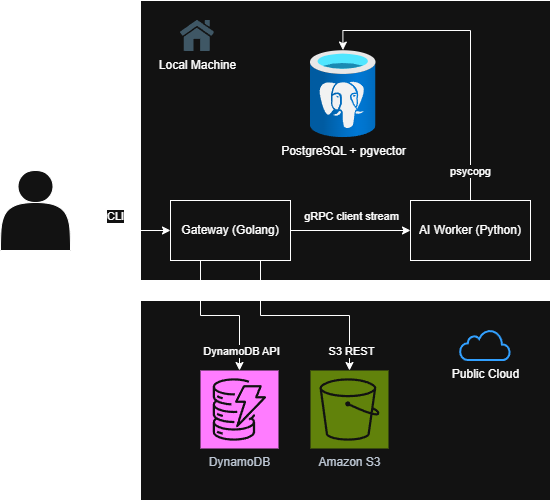
\includegraphics[width=0.5\linewidth]{HybridArchitectureDiagram.drawio.png}
	\caption{Architektura Hybrydowa}
\end{figure}

\begin{itemize}
    \item \textbf{Gateway w Go:}
    obsługuje CLI, odczyt plików, obliczanie skrótów i sterowanie
    potokiem. Wywołuje AI Workera oraz interfejsy S3 i DynamoDB.
    \item \textbf{AI Worker w Pythonie:}
    odbiera obrazy, dla których nie potwierdzono duplikatu binarnego.
    Wyznacza reprezentację i ocenę jakości, wyszukuje odpowiednik
    w PostgreSQL, a następnie zwraca wynik decyzji.
\end{itemize}

Warstwę danych podzielono według rodzaju informacji.
Interfejs S3 wykorzystano do zapisu obrazów i osobnych obiektów JSON,
DynamoDB do przechowywania metadanych plików i indeksu par skrótów, a PostgreSQL
z rozszerzeniem \texttt{pgvector} do przechowywania i przeszukiwania
reprezentacji wektorowych. Rozdzielenie tych zadań wykorzystuje
odpowiednio model obiektowy, odczyty według klucza i operacje
na wektorach~\cite{aws_s3_welcome_doc,awsGetItem,pgvector_docs}.
Wektory są zapisywane bezpośrednio przez AI Workera.
Nie są zwracane bramie.

Nazwę bazową pliku, uzyskaną przez \texttt{filepath.Base}, przyjęto
jako identyfikator aplikacyjny. Obraz zapisywany jest pod kluczem
\texttt{payloads/\allowbreak<file\_name>}, a jego opis pod
\texttt{metadata/\allowbreak<file\_name>.json}.
Opis JSON jest osobnym obiektem, nie zestawem metadanych użytkownika
dołączonych do obiektu obrazu.
W DynamoDB zastosowano dwa rodzaje rekordów:

\begin{itemize}
    \item \textbf{Rekord metadanych pliku:}
    \texttt{PK = FILE\#<file\_name>}, \texttt{SK = META};
    rekord zawiera m.in. klucz obiektu, rozmiar, wymiary i skróty.
    \item \textbf{Indeks zawartości:}
    \texttt{PK = CHUNK\#<c>}, \texttt{SK = FULL\#<h>};
    rekord wiąże skrót pierwszego fragmentu i całego pliku
    z zapisanym obiektem.
\end{itemize}

Osobno obsługiwane są powtarzające się nazwy bazowe w jednym
przetwarzanym zbiorze. Przed uruchomieniem zadań zachowywane jest
pierwsze wystąpienie, a następne zgłaszane są jako błędy wejścia.
Takie zachowanie wynika z przyjęcia nazwy bazowej jako identyfikatora,
również dla plików pochodzących z różnych katalogów.

\subsubsection{Dobór technologii: Go oraz Python}

Go wykorzystano do obsługi I/O i organizacji współbieżnego przetwarzania.
Goroutines są rozdzielane przez środowisko wykonawcze między wątki
systemowe; blokowanie podczas I/O nie musi zatrzymywać pozostałych
goroutines~\cite{go_effective}.
Mechanizm ten nie zastępuje synchronizacji współdzielonego stanu,
dlatego równoległość bramy ograniczono jawnie, jak opisano
w podrozdziale~\ref{subsec:wspolbieznosc}.

Python wykorzystano w części analitycznej z PyTorch.
Oficjalne repozytorium SSCD udostępnia modele TorchScript i przykłady
inferencji w tym środowisku~\cite{sscd_repo}.
Rozdzielenie usług pozwala zmieniać przygotowanie obrazu i inferencję
bez przenoszenia tej logiki do kodu obsługującego magazyny danych.
W badanej wersji model ładowany jest na CPU.

\subsubsection{Komunikacja za pomocą gRPC}
\label{subsubsec:grpc-komunikacja}

Kontrakt zdefiniowano w pliku \texttt{proto/dedup.proto}.
Na podstawie definicji usługi i wiadomości wygenerowano kod dla obu
języków, zgodnie z modelem pracy gRPC~\cite{grpc_core_concepts}.
Wykorzystany transport HTTP/2 obsługuje wiele strumieni w jednym
połączeniu; nie oznacza to jednak, że obiekt klienta musi utrzymywać
zawsze dokładnie jedno połączenie TCP~\cite{rfc9113,grpc_go_client}.

\begin{lstlisting}[
    language={},
    basicstyle=\ttfamily\small,
    numbers=left,
    firstnumber=1,
    breaklines=true,
    caption={Fragment kontraktu dedup.proto. Opracowanie własne.},
    label={lst:dedup-proto}
]
service ImageDedupService {
  rpc ProcessImageStream(stream ImageChunk)
      returns (ProcessImageResponse);
}

message ImageChunk {
  string image_key = 1;
  int64 total_size = 2;
  bytes data = 3;
  float threshold = 4;
}

message ProcessImageResponse {
  string status = 1;
  string image_key = 2;
  float quality_score = 3;
  float distance = 4;
  string existing_image_key = 5;
}
\end{lstlisting}

Metoda \texttt{ProcessImageStream} jest wywołaniem ze strumieniowaniem
po stronie klienta. Przesyłana jest sekwencja wiadomości
\texttt{ImageChunk}, po której odbierana jest pojedyncza odpowiedź;
gRPC zachowuje kolejność wiadomości w obrębie tego
wywołania~\cite{grpc_core_concepts}.
Pole \texttt{bytes} w Protocol Buffers przenosi dane binarne
z zakodowaną długością, bez konieczności zamiany obrazu
na tekst~\cite{protobuf_encoding}.

W bramie tworzony jest jeden współdzielony \texttt{grpc.ClientConn}.
Jest to kanał klienta, a nie zaimplementowana w aplikacji pula
połączeń~\cite{grpc_go_client}.
Adres określa zmienna
\texttt{AI\_\allowbreak WORKER\_\allowbreak GRPC\_\allowbreak ADDR},
domyślnie \texttt{localhost:50051}; w Docker Compose wskazano usługę
AI Workera. W tej konfiguracji nie zastosowano TLS ani osobnego
limitu czasu dla każdego RPC.
Brak jawnego terminu wywołania oznacza, że samo gRPC nie narzuca
takiego ograniczenia~\cite{grpc_deadlines}.

Stan transportu odróżniono od pola aplikacyjnego \texttt{status}.
Błędy RPC przekazywane są kodami gRPC, natomiast pole wiadomości
opisuje wynik deduplikacji~\cite{grpc_status_codes}.
AI Worker jawnie zwraca \texttt{INVALID\_ARGUMENT}, gdy nie otrzyma
klucza obrazu albo danych. Nie zaimplementowano pełnej walidacji
zadeklarowanego rozmiaru ani zakresu wartości progu.

\subsection{Logiczny potok deduplikacyjny}
\label{subsec:logiczny-potok}

Przed uruchomieniem potoku odczytywane są rozmiar pliku i konfiguracja
obrazu. Niepowodzenie dekodowania, w tym próba odczytu pustego pliku,
kończy przetwarzanie przed CDC i RPC.
W potoku zastosowano trzy etapy. Najpierw wykonywany jest
\texttt{ChunkPipeline}, następnie \texttt{FullHashPipeline},
a na końcu \texttt{SimilarityPipeline}.
Każdy zwraca decyzję \texttt{continue}, \texttt{accept\_full}
albo \texttt{soft\_dedup}. Pierwsza decyzja inna niż
\texttt{continue}, podobnie jak błąd, kończy wykonanie łańcucha.

Etapy jednego pliku wykonywane są sekwencyjnie; współbieżnie
przetwarzane są różne pliki.
Nie zbudowano oddzielnych procesów roboczych połączonych kanałami
dla każdego etapu. Jest to rozróżnienie względem potoków Go,
w których równoległe grupy goroutines przekazują dane przez
kanały~\cite{go_pipelines}.
Pominięcie dalszej analizy wynika z otrzymanej decyzji,
nie z założenia, że każdy kolejny etap musi trwać dłużej.

\subsubsection{Wstępne wyszukiwanie z wykorzystaniem CDC}
\label{subsubsec:potok-cdc}

Porcjowanie zależne od treści (ang. \textit{Content-Defined Chunking},
CDC) wyznacza granice fragmentów na podstawie danych, a nie wyłącznie
pozycji bajtów. Ogranicza przez to skutki przesunięcia granic po
wstawieniu lub usunięciu części zawartości, występujące w podziale
na bloki o stałej długości~\cite{gregoriadis2024cdc}.
W tym projekcie użyto tylko pierwszego fragmentu jako filtra
kandydatów. Nie zaimplementowano przechowywania i deduplikowania
wszystkich fragmentów pliku.

Zastosowano bibliotekę \texttt{restic/chunker} w wersji
\texttt{v0.5.0}, wykorzystującą kroczący odcisk
Rabina~\cite{restic2026chunker}.
Odcisk aktualizowany jest dla przesuwanego okna i służy do wyznaczenia
granicy, a nie do kryptograficznej identyfikacji
zawartości~\cite{gregoriadis2024cdc}.
W użytej wersji okno ma \(64\) bajty, a domyślny warunek podziału
sprawdza \(20\) najmłodszych bitów odcisku~\cite{restic2026code}.
W aplikacji ustawiono stały wielomian
\texttt{0x3DA3358B4DC173} stopnia \(53\).

Domyślne progi biblioteki wynoszą \(512\,\mathrm{KiB}\)
i \(8\,\mathrm{MiB}\), a parametr nominalnego średniego rozmiaru
odpowiada \(1\,\mathrm{MiB}\)~\cite{restic2026chunker,restic2026code}.
Dolny próg ogranicza poszukiwanie granicy, górny wymusza zakończenie
fragmentu; koniec pliku pozwala zwrócić również krótszy
fragment~\cite{restic2026code}.
Nominalny parametr nie gwarantuje takiej samej średniej w badanym
zbiorze danych~\cite{gregoriadis2024cdc}.

Implementacja przewiduje ponadto odczyt zastępczy.
Gdy sprawdzenie stopnia wielomianu nie przejdzie albo biblioteka
nie zwróci poprawnego, niepustego fragmentu, plik jest przewijany
do początku i odczytywane jest do \(64\,\mathrm{KiB}\).
Nie jest to wówczas podział CDC.
Bufor początkowy tej samej wielkości przekazywany do biblioteki
nie ogranicza prawidłowego fragmentu CDC do \(64\,\mathrm{KiB}\).

Niech \(C_1(f)\) oznacza fragment rzeczywiście zwrócony przez
\texttt{readFirstChunk}: pierwszy fragment CDC albo, w ścieżce
zastępczej, prefiks długości \(\min(|f|,64\,\mathrm{KiB})\).
Zdefiniowano dwa identyfikatory:

\begin{equation}
\label{eq:cdc-hashes}
c=\operatorname{SHA256}\!\left(C_1(f)\right),
\qquad
h=\operatorname{SHA256}(f).
\end{equation}

Definicję funkcji SHA-256 określa standard
FIPS~180-4~\cite{shs2015}.
Równanie~\eqref{eq:cdc-hashes} jest natomiast oznaczeniem przyjętym
w projekcie i nie zakłada jednoczesnego obliczenia obu skrótów.
W zwykłej ścieżce CDC plik krótszy niż \(512\,\mathrm{KiB}\)
stanowi cały pierwszy fragment; wtedy \(c=h\).
W ścieżce zastępczej taka równość wynika z objęcia całego pliku
prefiksem tylko dla rozmiaru nieprzekraczającego \(64\,\mathrm{KiB}\).

Po wyznaczeniu \(c\) wykonywana jest operacja \texttt{Query}
dla \texttt{PK = CHUNK\#<c>} z parametrem \texttt{Limit = 1}.
Limit ogranicza liczbę ocenianych elementów, nie stanowi ogólnej
gwarancji uzyskania jednego dopasowania po zastosowaniu
filtra~\cite{awsQuery}.
W badanym kodzie nie użyto \texttt{FilterExpression}, dlatego
obecność zwróconego elementu wystarcza do wskazania kandydata.
Wynik zapisywany jest we fladze \texttt{ChunkMatched}.

\begin{figure}[!htbp]
\centering
\begin{lstlisting}[
    language={},
    frame=single,
    basicstyle=\ttfamily\small,
    breaklines=true
]
c = sha256(readFirstChunk(file))
Query PK = CHUNK#c, Limit = 1
  miss -> skip exact full-hash lookup; similarity
  hit:
    h = sha256(file)
    GetItem PK = CHUNK#c, SK = FULL#h
      hit  -> binary soft-dedup
      miss -> similarity
\end{lstlisting}
\caption{Dwuetapowe wyszukiwanie duplikatu binarnego.
Opracowanie własne na podstawie implementacji.}
\label{fig:cdc-lookup-algo}
\end{figure}

\subsubsection{Weryfikacja pełnego skrótu i warunki kontynuacji}
\label{subsubsec:potok-full-hash}

Trafienie dla \(c\) nie potwierdza tożsamości plików.
Mogą one zawierać taki sam początkowy fragment i różnić się dalszą
zawartością. Nie jest to kolizja funkcji skrótu, ponieważ haszowany
fragment jest w obu przypadkach identyczny.
Po trafieniu plik otwierany jest ponownie, a \(h\) obliczane
z całej zawartości, łącznie z wcześniej odczytanym początkiem.

Następnie wykonywane jest \texttt{GetItem} dla
\texttt{PK = CHUNK\#<c>} i \texttt{SK = FULL\#<h>}.
Operacja odczytuje rekord po pełnym kluczu głównym, obejmującym
w tej tabeli klucz partycji i klucz sortowania~\cite{awsGetItem}.
Trafienie kończy łańcuch decyzją \texttt{soft\_dedup}.
Nie uruchamia się RPC ani zapisu kolejnej kopii obrazu.
Nadal zapisywany jest jednak obiekt JSON z metadanymi przetwarzania.

Niech \(\mathcal{I}\) oznacza ustalony zbiór par skrótów
\((c',h')\) w indeksie, a
\(\mathcal{C}=\{c'\mid \exists h':(c',h')\in\mathcal{I}\}\)
zbiór skrótów początkowych fragmentów.
Warunek rozpoznania duplikatu w gałęzi binarnej zapisano jako:

\begin{equation}
\label{eq:soft-dedup}
\operatorname{dup}_{\mathrm{bin}}(f)
\iff (c,h)\in\mathcal{I}.
\end{equation}

Jest to formalizacja schematu indeksowania, nie wzór zaczerpnięty
z definicji CDC. Obecność pary implikuje obecność \(c\)
w \(\mathcal{C}\), więc pierwsze zapytanie pozwala odroczyć
obliczenie \(h\), zamiast dostarczać osobnego kryterium tożsamości.
Predykatu \(\operatorname{dup}_{\mathrm{bin}}\) nie utożsamiono
z każdą decyzją \texttt{soft\_dedup}.
Dotyczy ona także statusu \texttt{duplicate\_rejected}
z gałęzi podobieństwa.
Zgodność skrótów przyjęto jako kryterium projektu, bez porównywania
plików bajt po bajcie i bez zakładania matematycznej niemożliwości
kolizji.

Jeżeli odczyty zakończą się poprawnie, kontynuacja do analizy
podobieństwa odpowiada warunkowi:

\begin{equation}
\label{eq:full-hash-continue}
\operatorname{continue}_{\mathrm{bin}}(f)
\iff
(c\notin\mathcal{C})
\;\lor\;
\bigl(c\in\mathcal{C}\land(c,h)\notin\mathcal{I}\bigr).
\end{equation}

W wykonaniu stosowana jest ocena warunkowa.
Brak kandydata pozwala przejść do analizy podobieństwa bez obliczania
\(h\) na potrzeby wyszukania duplikatu. Nie oznacza to pominięcia
pełnego skrótu przez cały proces: jeśli obraz zostanie zaakceptowany
do zapisu, brakujące \(h\) jest obliczane w \texttt{uploadImage}
przed przesłaniem danych i utworzeniem wpisu indeksu.

\begin{figure}[!htbp]
\centering
\begin{lstlisting}[
    language={},
    frame=single,
    basicstyle=\ttfamily\small,
    breaklines=true
]
no CHUNK#c:
  similarity without full hash in lookup stage
  accepted -> compute missing full hash before upload

CHUNK#c exists, no matching FULL#h:
  similarity with full hash already available
\end{lstlisting}
\caption{Dwie ścieżki kontynuacji po niepotwierdzeniu duplikatu.
Opracowanie własne na podstawie implementacji.}
\label{fig:full-hash-continue-algo}
\end{figure}

W kodzie nie ustawiono \texttt{ConsistentRead}.
W usłudze DynamoDB oznacza to domyślnie spójność ostateczną:
odczyt może nie uwzględniać niedawnego zapisu~\cite{aws_read_consistency}.
Równania~\eqref{eq:soft-dedup} i~\eqref{eq:full-hash-continue}
opisują regułę dla ustalonego stanu indeksu, nie atomowy obraz
dwóch kolejnych wywołań.
Brak trafienia oznacza zatem niepotwierdzenie duplikatu
w odczytanym stanie, a nie bezwarunkową gwarancję unikalności.

\subsection{Integracja z modułem analitycznym i obsługa wyników}
\label{subsec:similarity-grpc-pipeline}

\subsubsection{Przesłanie i buforowanie obrazu}

Po niepotwierdzeniu duplikatu binarnego plik otwierany jest ponownie
i przesyłany od początku metodą \texttt{ProcessImageStream}
usługi \texttt{dedup.v1.ImageDedupService}.
Podział transportowy jest niezależny od CDC.
W kliencie zastosowano bufor o pojemności
\(B=2\,\mathrm{MiB}=2\cdot2^{20}\) bajtów.
Każdy dodatni wynik wywołania \texttt{Read} wysyłany jest
w osobnej wiadomości.

Interfejs \texttt{io.Reader} dopuszcza odczyt krótszy od pojemności
bufora, także przed końcem danych~\cite{go_io_reader}.
Dla poprawnie przesłanego niepustego pliku, bez wcześniejszego
zakończenia strumienia, oznaczono przez \(b_i\) liczbę bajtów obrazu
w wiadomości \(i\), a przez \(s\) rozmiar pliku.
Wówczas:

\begin{equation}
\label{eq:message-count}
\sum_{i=1}^{n}b_i=s,\qquad
0<b_i\leq B
\quad\Longrightarrow\quad
n\geq\left\lceil\frac{s}{B}\right\rceil.
\end{equation}

Równość zachodzi, gdy wszystkie wiadomości poza ostatnią zawierają
pełne \(B\) bajtów danych. Nie jest to gwarancja obecnej implementacji,
ponieważ nie zastosowano dopełniania krótkich odczytów przez
\texttt{io.ReadFull}~\cite{go_io_reader}.
Równanie wynika z przyjętej pojemności bufora, a nie z właściwości
algorytmu CDC.

Pierwsza wiadomość zawiera dane obrazu oraz pola
\texttt{image\_key}, \texttt{total\_size} i \texttt{threshold}.
W kolejnych wiadomościach wypełniane jest tylko \texttt{data}.
Limit odbioru i wysyłania po stronie AI Workera ustawiono na
\(8\,\mathrm{MiB}\) na wiadomość.
Limit wiadomości gRPC nie ogranicza łącznego rozmiaru strumienia,
a do danych obrazu dochodzi narzut kodowania pól
Protocol Buffers~\cite{grpc_core_limits,protobuf_encoding}.

Po stronie odbiorcy użyto \texttt{SpooledTemporaryFile}
z progiem \(20\,\mathrm{MiB}\).
Po jego przekroczeniu bufor przechodzi z pamięci operacyjnej do pliku
tymczasowego~\cite{python_tempfile}.
AI Worker zbiera cały strumień, a dopiero potem uruchamia ocenę
jakości i inferencję. Strumieniowy transport nie oznacza więc
inferencji na niekompletnym obrazie.
Próg bufora nie jest też limitem całkowitej pamięci procesu,
ponieważ poza nim przechowywane są model i zdekodowane dane obrazu.

Jeżeli \texttt{Send} zwróci \texttt{io.EOF}, klient kończy wysyłanie
i wywołuje \texttt{CloseAndRecv}, aby odebrać wynik lub końcowy
status RPC. Jest to zgodne z możliwością zakończenia wywołania
przez serwer przed odebraniem wszystkich wiadomości
klienta~\cite{grpc_core_concepts}.
Inne błędy wysyłania przerywają przetwarzanie.

\subsubsection{Decyzja AI Workera}

Pole \texttt{threshold} przenosi maksymalną dopuszczalną odległość
kosinusową, domyślnie \(0{,}60\), a nie minimalne podobieństwo.
W zapytaniu do \texttt{pgvector} użyto operatora \texttt{<=>};
odpowiada on odległości kosinusowej, podczas gdy podobieństwo
wynosi jeden minus ta odległość~\cite{pgvector_docs}.
Definicję reprezentacji i dobór progu przedstawiono
w podrozdziałach~\ref{sec:reprezentacja-wektorowa}
i~\ref{sec:ewaluacja-progów}.

AI Worker wykonuje wyszukanie i ewentualną aktualizację
PostgreSQL przed zwróceniem odpowiedzi RPC.
Odpowiedź zawiera identyfikatory, ocenę jakości i odległość,
ale nie reprezentację wektorową.
W bramie status mapowany jest na dalsze działanie:

\begin{itemize}
    \item \textbf{\texttt{inserted}:}
    przyjmowany jest zapis obrazu.
    W PostgreSQL użyto operacji \texttt{INSERT ... ON CONFLICT},
    więc status nie gwarantuje utworzenia nowego wiersza przy
    ponownym użyciu tego samego \texttt{image\_key}.
    \item \textbf{\texttt{duplicate\_rejected}:}
    zwracana jest decyzja \texttt{soft\_dedup}.
    Pomijany jest zapis obrazu i wpisów DynamoDB, ale zapisywany
    jest obiekt JSON.
    \item \textbf{\texttt{replaced}:}
    przyjmowany jest zapis obrazu i ustawiana flaga
    \texttt{ReplaceExisting}. Rekord PostgreSQL aktualizowany
    jest w miejscu przez \texttt{UPDATE}, bez poprzedzającego
    \texttt{DELETE}.
\end{itemize}

\subsubsection{Kolejność zapisu i wycofanie poprzedniej wersji}

Po poprawnym zakończeniu łańcucha serializowany i zapisywany jest JSON.
Przy \texttt{soft\_dedup} proces kończy się na tym etapie.
Dla zaakceptowanego obrazu najpierw uzupełniany jest brakujący pełny
skrót. Następnie obraz zapisywany jest pod kluczem
\texttt{payloads/\allowbreak<file\_name>}.
Na końcu zapisywane są rekord metadanych pliku
\texttt{FILE\#\allowbreak<file\_name>/\allowbreak META}
i para \texttt{CHUNK\#<c>/\allowbreak FULL\#<h>}.
Są to oddzielne operacje, a nie jedna transakcja.

Funkcja \texttt{retireReplaced} uruchamiana jest dopiero po
poprawnym zapisaniu nowego obrazu i obu wpisów indeksu.
Jeżeli \texttt{existing\_image\_key} różni się od nowej nazwy,
odczytywany jest stary rekord metadanych pliku, a następnie usuwane są:
poprzedni obraz, jego JSON, rekord metadanych oraz, jeśli odczytano
potrzebne skróty, rekord zawartości.
Przy identycznym kluczu osobne usuwanie jest pomijane.
Żadna z tych ścieżek nie usuwa lokalnego pliku źródłowego.

Skrypt inicjalizacyjny nie włącza wersjonowania zasobnika.
Nie należy jednak utożsamiać tego z gwarancją konfiguracji każdego
środowiska, do którego zostanie podłączona brama.
Przy włączonym wersjonowaniu S3 ponowny zapis pod tym samym kluczem
tworzy nową wersję, a usunięcie bez identyfikatora wersji dodaje
znacznik usunięcia zamiast kasować wcześniejsze
wersje~\cite{aws_s3_versioning_workflows}.

Dla statusu \texttt{replaced} rozmiar poprzedniego obrazu
odczytywany jest przez \texttt{HeadObject}.
Niech \(k_{\mathrm{old}}\) i \(k_{\mathrm{new}}\) oznaczają klucze,
a \(s_{\mathrm{old}}\) i \(s_{\mathrm{new}}\) rozmiary w bajtach.
Licznik projektu ma postać:

\begin{equation}
\label{eq:deleted-bytes}
\texttt{deleted\_bytes}=
\begin{cases}
0, & \text{gdy odczyt rozmiaru nie powiedzie się},\\
\max(0,s_{\mathrm{old}}-s_{\mathrm{new}}),
    & \text{gdy }k_{\mathrm{old}}=k_{\mathrm{new}},\\
s_{\mathrm{old}},
    & \text{gdy }k_{\mathrm{old}}\neq k_{\mathrm{new}}.
\end{cases}
\end{equation}

Dwie ostatnie gałęzie zakładają poprawny odczyt rozmiaru.
Przy tym samym kluczu liczona jest dodatnia różnica rozmiarów,
przy różnych kluczach cały rozmiar poprzedniego obiektu.
Nie jest to zatem jednolita miara oszczędności netto.
Ponadto S3 rozlicza zachowane wersje jako pełne obiekty,
nie różnice między wersjami~\cite{aws_s3_versioning_workflows}.
Interpretację kosztową pozostawiono analizie
w rozdziale~\ref{chap:ewaluacja-i-finops}.

\subsection{Miejsce oceny jakości w potoku}
\label{subsec:logika-decyzyjna}

Ocenę podobieństwa oddzielono od wyboru przechowywanej wersji.
Pierwsza wskazuje kandydata, druga rozstrzyga decyzję obsługiwaną
przez AI Workera. W bramie nie występuje osobny etap
\texttt{InfoGain}; klasa \texttt{SimilarityPipeline} odbiera
gotowy status i ustawia decyzję zapisu.
Plik \texttt{decision.go} definiuje możliwe decyzje potoku,
nie algorytm oceny jakości.

Wynik oceny przekazywany jest w polu \texttt{quality\_score}.
Pole \texttt{existing\_image\_key} wskazuje obiekt podlegający
ewentualnemu wycofaniu.
Definicję wskaźnika, kierunek porównania i obsługę remisu przedstawiono
w podrozdziale~\ref{sec:infogain-jakosc}.

\subsection{Współbieżność i zakres gwarancji spójności}
\label{subsec:wspolbieznosc}

\subsubsection{Limity i anulowanie pracy}

Do ograniczenia współbieżności użyto pakietu \texttt{errgroup}.
Grupę tworzono przez \texttt{WithContext}, a limit ustawiano
metodą \texttt{SetLimit}.
Parametr \texttt{--workers} ma domyślną wartość \(10\);
przyjęto co najmniej jedno zadanie.
\texttt{SetLimit} ogranicza liczbę aktywnych goroutines grupy,
a dodanie następnej może oczekiwać na zwolnienie
miejsca~\cite{go_errgroup}.
Nie jest to stała pula połączona kolejką aplikacyjną.

Wewnętrznie \texttt{errgroup} może anulować kontekst po zwróceniu
pierwszego błędu przez zadanie~\cite{go_errgroup}.
W tej aplikacji błędy pojedynczych obrazów są jednak rejestrowane,
a funkcja zadania zwraca \texttt{nil}.
Niepowodzenie jednego pliku nie przerywa więc automatycznie całego
zbioru; po zakończeniu zliczane są nieudane operacje.
Kontekst obsługuje natomiast przerwanie przez \texttt{SIGINT}
lub \texttt{SIGTERM}.

AI Worker wykorzystuje \texttt{ThreadPoolExecutor} z limitem
czterech wątków obsługi gRPC.
Przed rozpoczęciem przyjmowania wywołań inicjalizowany jest schemat
bazy i ładowany model.
Limit ten jest niezależny od liczby zadań bramy i nie stanowi
gwarancji czterokrotnego przyspieszenia inferencji.
Próg buforowania \(20\,\mathrm{MiB}\) dotyczy pojedynczego
strumienia, nie sumy danych wszystkich żądań.

\subsubsection{Transakcja decyzji i operacje między magazynami}

W \texttt{Repository.resolve} otwierana jest transakcja PostgreSQL.
Następnie pobierana jest blokada
\texttt{pg\_\allowbreak advisory\_\allowbreak xact\_\allowbreak lock}
ze stałym identyfikatorem \(74821001\).
Transakcyjne blokady doradcze są zwalniane na końcu transakcji
i wymagają współpracy aplikacji używających tej samej
konwencji~\cite{postgres16_locking}.
Wspólny identyfikator szereguje całe sekcje rozstrzygania decyzji
w tej samej bazie, również dla różnych obrazów.
Blokada nie obejmuje wcześniejszego obliczania reprezentacji
i jakości.

Przy odczycie jakości istniejącego obrazu stosowane jest także
\texttt{SELECT ... FOR UPDATE}.
Taka blokada chroni wskazany wiersz przed konkurencyjną modyfikacją
do końca transakcji~\cite{postgres16_locking}.
Wyjście z kontekstu transakcji Psycopg kończy się zatwierdzeniem
albo wycofaniem zmian zależnie od wystąpienia
wyjątku~\cite{psycopg_transactions}.
Zatwierdzenie następuje przed zwróceniem odpowiedzi do bramy.

Ochrona PostgreSQL nie obejmuje późniejszych zapisów JSON, obrazu
i indeksów DynamoDB. W kodzie nie zastosowano wspólnej transakcji,
zapisów warunkowych DynamoDB ani procedury kompensacji po błędzie.
Przerwanie po aktualizacji PostgreSQL może zatem pozostawić
rekord wektorowy bez odpowiadającego mu nowego obrazu;
przerwanie kolejnych zapisów może pozostawić niepełny indeks.
Nie można na tej podstawie zadeklarować atomowej podmiany
we wszystkich magazynach.

Pozostaje też ograniczenie podmiany pod tą samą nazwą.
\texttt{retireReplaced} pomija wtedy czyszczenie, mimo że nowy zapis
może dotyczyć innych skrótów. Stary rekord
\texttt{CHUNK\#<c>/\allowbreak FULL\#<h>} może nadal wskazywać nadpisany obiekt.
Z tego względu poprawność kolejnego trafienia binarnego zależy
również od aktualności indeksu, a nie wyłącznie od zgodności
skrótów. Ograniczenie to wymaga usunięcia w implementacji
lub uwzględnienia w ocenie wyników.

% \subsection{Perspektywa docelowa: wdrożenie chmurowe w AWS}
% \label{subsec:architektura-cloud-native}

% Przeniesienie analizy z urządzenia klienta do AWS stanowi wariant
% rozwojowy. Poniżej przedstawiono jego założenia i ograniczenia,
% nie wyniki wdrożenia. Wariant z instancjami EC2 nie jest traktowany
% jako rozwiązanie w całości bezserwerowe.

% \subsubsection{Model operacyjny i punkt wejścia CLI}
% \label{subsubsec:cloud-cli}

% CLI może pozostać punktem wejścia uruchamianym lokalnie, natomiast
% analiza obrazu może zostać przeniesiona do usług chmurowych.
% Wymaga to ustalenia miejsca deduplikacji względem pierwszego zapisu.
% Jeżeli analiza jest uruchamiana dopiero po zapisaniu obiektu
% w S3, nie eliminuje tego początkowego transferu ani operacji zapisu.
% Nie jest więc funkcjonalnie równoważna obecnemu filtrowaniu
% przed wysłaniem pliku do magazynu.
% % TODO[ARCH-14]: Wybrać wariant: analiza przed zapisem docelowym
% % albo zapis w obszarze tymczasowym i późniejsze przetwarzanie.

% \subsubsection{Asynchroniczne przetwarzanie z wykorzystaniem Amazon SQS}
% \label{subsubsec:cloud-sqs}

% W wariancie po zapisie można wykorzystać powiadomienia o utworzeniu
% obiektu S3 kierowane do kolejki Amazon SQS~\cite{aws_s3_events}.
% Kolejka standardowa dostarcza wiadomości co najmniej raz
% i może zmienić ich kolejność~\cite{aws_sqs_standard}.
% Projekt konsumenta musi zatem uwzględniać ponowne otrzymanie zdarzenia
% oraz zdarzenia dotyczące różnych wersji obiektu.
% Zastąpienie synchronicznego RPC takim przepływem wymaga również
% określenia sposobu odbioru wyniku przez CLI.
% % TODO[ARCH-15]: Określić identyfikację zadania, idempotencję,
% % ponowienia, obsługę błędów i sposób raportowania wyniku użytkownikowi.

% \subsubsection{Warstwa obliczeniowa AI: AWS Lambda lub EC2 z GPU}
% \label{subsubsec:cloud-ai-compute}

% Do dalszej oceny przewidziano AWS Lambda i instancje EC2 z GPU.
% Dobór wariantu Lambda wymaga sprawdzenia limitów czasu wykonania
% i pamięci w danym trybie usługi~\cite{aws_lambda_quotas}.
% AWS udostępnia także instancje EC2 z akceleratorami GPU,
% które mogą stanowić środowisko obliczeniowe modułu
% analitycznego~\cite{aws_ec2_accelerated}.
% Wybór powinien wynikać z pomiarów czasu inicjalizacji modelu,
% inferencji i wykorzystania zasobów, a nie z samej nazwy usługi.
% % TODO[ARCH-16]: Zmierzyć cold start, przepustowość i koszt.
% % Uzasadnienie wyboru wobec Amazon Bedrock pozostawić do czasu
% % określenia konkretnej usługi, modelu i wymagań inferencji.

% \subsubsection{Warstwa danych: DynamoDB i Aurora PostgreSQL}
% \label{subsubsec:cloud-data-layer}

% Wariant chmurowy może zachować S3 jako magazyn obiektów
% i DynamoDB jako indeks skrótów.
% Aurora PostgreSQL obsługuje rozszerzenie \texttt{pgvector}
% oraz wyszukiwanie wektorowe w wariancie Serverless
% v2~\cite{aws_aurora_vectors}.
% Samo przeniesienie bazy nie rozstrzyga jednak wyboru indeksu
% wektorowego: \texttt{pgvector} oferuje wyszukiwanie dokładne
% oraz indeksy przybliżone HNSW i IVFFlat~\cite{pgvector_docs}.
% Konfiguracja docelowa wymaga więc osobnej oceny jakości wyszukiwania,
% opóźnienia i kosztu.
% % TODO[ARCH-17]: Ustalić wersję silnika i rozszerzenia, typ indeksu,
% % konfigurację połączeń oraz parametry skalowania.

\clearpage % Rozdziały zaczynamy od nowej strony.
\section{Moduł sztucznej inteligencji i analiza semantyczna obrazów}

Rozdział opisuje warstwę AI Workera, która rozpoznaje duplikaty
percepcyjne. Są to pliki o innej zawartości bajtowej, ale o tej samej
treści wizualnej, np. ponownie skompresowane, przeskalowane lub
przycięte kopie. Funkcje skrótu kryptograficznego nie wykrywają takich
par, ponieważ zmiana kodowania obrazu daje inny skrót
pliku~\cite{pizzi2022sscd}.

Moduł składa się z trzech części: ekstrakcji wektora cech modelem SSCD,
wyszukiwania najbliższego sąsiada w PostgreSQL z rozszerzeniem
\texttt{pgvector} oraz bezreferencyjnej oceny jakości. Podstawy
teoretyczne, czyli GeM, funkcję straty InfoNCE, regularyzację KoLeo
i miarę kosinusową, przedstawiono w rozdziale~2. Transport gRPC,
buforowanie strumienia i mapowanie statusów w bramie opisano
w podrozdziale~\ref{subsec:similarity-grpc-pipeline}. Poniżej
uwzględniono tylko elementy potrzebne do zrozumienia decyzji
podejmowanej przez AI Workera.

W całym rozdziale fakty o implementacji pochodzą z kodu repozytorium
\texttt{s3-dedup-engine}. Wnioski, które nie zostały zmierzone,
oznaczono jako przypuszczenia.

% ------------------------------------------------------------------
\subsection{Ekstrakcja cech i model SSCD (Self-Supervised Descriptor)}
\label{sec:model-sscd}

\subsubsection{Wykrywanie kopii a klasyfikacja obrazów}

Zadanie wykrywania kopii różni się od klasyfikacji. Autorzy SSCD
przyjmują, że dwa obrazy są kopiami wtedy i tylko wtedy, gdy pochodzą
z tego samego dwuwymiarowego źródła~\cite{pizzi2022sscd}.
Dwa różne zdjęcia tego samego psa nie są więc kopiami, mimo że należą
do tej samej klasy. Wektor odpowiedni dla klasyfikacji powinien
zbliżać obrazy jednej klasy. Wektor do wykrywania kopii powinien
natomiast utrzymywać w oddaleniu nawet obrazy semantycznie podobne,
a całą przestrzeń wypełniać możliwie równomiernie~\cite{pizzi2022sscd}.

Z tego powodu sieci wytrenowane z nadzorem na zbiorze
ImageNet~\cite{deng2009imagenet} nie są dobrym wyborem do tego zadania.
Uczą się one niezmienniczości względem cech, które nie zmieniają klasy
obiektu. W deduplikacji ta sama niezmienniczość prowadziłaby do
łączenia różnych zdjęć o podobnej treści. Tabela~\ref{tab:sscd-uap}
zestawia wyniki z pracy SSCD na zbiorze DISC2021.
Miara \(\mu\mathrm{AP}\) jest polem pod krzywą precyzja--czułość
wyznaczoną dla wszystkich par zwróconych przez system, łącznie
dla wszystkich zapytań~\cite{douze2021disc}. Odpowiada to stosowaniu
jednego, wspólnego progu odległości dla całego
zbioru~\cite{pizzi2022sscd}, czyli warunkom pracy bramy.

\begin{table}[!htbp]
\centering
\caption{Skuteczność wybranych deskryptorów w wykrywaniu kopii na
zbiorze DISC2021. \(\mu\mathrm{AP}_{SN}\) oznacza wynik po normalizacji
podobieństwa zbiorem tła. Opracowanie własne na podstawie
\cite{pizzi2022sscd}.}
\label{tab:sscd-uap}
\begin{tabular}{|l|r|r|r|}
\hline
\textbf{Model} & \textbf{Wymiar} & \(\boldsymbol{\mu\mathrm{AP}}\) [\%]
& \(\boldsymbol{\mu\mathrm{AP}_{SN}}\) [\%] \\
\hline
Multigrain (ImageNet, nadzorowany) & 1500 & 16,5 & 36,5 \\
Multigrain (ImageNet, nadzorowany) & 2048 & 20,5 & 41,7 \\
DINO ViT-B/16 & 1500 & 32,2 & 53,8 \\
SimCLR, wyjście sieci bazowej & 2048 & 13,1 & 33,9 \\
SimCLR, warstwa rzutująca & 128 & 9,4 & 17,3 \\
SSCD (DISC, adv.+mixup) & 512 & 61,5 & 72,5 \\
\hline
\end{tabular}
\end{table}

Model SSCD osiąga wyższy wynik od pozostałych deskryptorów przy
mniejszym wymiarze wektora niż modele Multigrain. Autorzy podają, że
SSCD przewyższa SimCLR o 48 punktów procentowych
\(\mu\mathrm{AP}\)~\cite{pizzi2022sscd}. Mniejszy wymiar ma znaczenie
praktyczne: zmniejsza rozmiar wiersza w bazie wektorowej i koszt
porównania pary wektorów.

\subsubsection{Budowa modelu}

SSCD wykorzystuje sieć ResNet-50~\cite{he2016resnet} jako sieć bazową.
Mapa cech z ostatniego bloku jest agregowana operacją GeM z
parametrem \(p=3\)~\cite{radenovic2018gem,pizzi2022sscd}. Następnie
stosowana jest warstwa liniowa rzutująca wektor do 512 wymiarów
i normalizacja L2. W przeciwieństwie do SimCLR~\cite{chen2020simclr}
warstwa rzutująca nie jest odrzucana po treningu, tylko pozostaje
częścią potoku wnioskowania~\cite{pizzi2022sscd}. Pełna ścieżka
wnioskowania ma więc postać:

\begin{equation}
\label{eq:sscd-forward}
\mathbf{e}(I)=
\frac{W\,\mathrm{GeM}_{p=3}\!\left(F(I)\right)}
{\left\|W\,\mathrm{GeM}_{p=3}\!\left(F(I)\right)\right\|_2},
\qquad \mathbf{e}(I)\in\mathbb{R}^{512},
\end{equation}

gdzie \(F\) oznacza sieć bazową ResNet-50, a \(W\) macierz warstwy
rzutującej. GeM uśrednia każdy kanał po wszystkich położeniach
przestrzennych, więc długość wektora nie zależy od wysokości i
szerokości mapy cech~\cite{radenovic2018gem}. Pozwala to podawać
na wejście obrazy o różnych proporcjach boków bez kadrowania.

Model był trenowany metodą samonadzorowaną, bez etykiet klas.
Pary pozytywne powstają jako dwie losowe transformacje tego samego
obrazu~\cite{chen2020simclr,pizzi2022sscd}. W wariancie
\texttt{sscd\_disc\_mixup} zestaw rozszerzony
(ang. \textit{advanced augmentations}) uzupełniono o mieszanie
obrazów metodami mixup i cutmix, stosowanymi z prawdopodobieństwem
po 2,5\%~\cite{pizzi2022sscd}. Wklejenie fragmentu jednego obrazu
w drugi modeluje kopie częściowe, np. kolaże~\cite{pizzi2022sscd}.
Zbiór DISC2021 zawiera właśnie takie przekształcenia: nakładki
tekstu i emotikon, zmiany kolorów, rozmycie, kompresję JPEG,
kadrowanie, obroty, odbicia oraz osadzanie obrazu w zrzucie ekranu
aplikacji~\cite{douze2021disc}. Odpowiadają one modyfikacjom,
którym podlegają obrazy przesyłane ponownie do magazynu obiektowego.

\subsubsection{Implementacja w AI Workerze}

Model ładowany jest z pliku TorchScript
\texttt{sscd\_disc\_mixup.torchscript.pt}, pobieranego z repozytorium
Hugging Face \texttt{m3/sscd-copy-detection}~\cite{hf_m3_sscd}.
Repozytorium to nie jest publikowane przez autorów SSCD; jego opis
odsyła do oficjalnego repozytorium Meta~\cite{hf_m3_sscd,sscd_repo},
w którym udostępniono model o tej samej nazwie: ResNet-50,
rozszerzenia adv.+mixup, wektor 512-wymiarowy~\cite{sscd_repo}.
Funkcja \texttt{hf\_hub\_download} jest wywoływana bez parametru
\texttt{revision}. Wersja pliku nie jest więc przypięta do konkretnej
rewizji repozytorium. Dla powtarzalności wyników należałoby zapisać
skrót pliku wag lub identyfikator rewizji.

Model wczytywany jest funkcją \texttt{torch.jit.load} na procesor CPU
i przełączany w tryb ewaluacji. Obiekt \texttt{SscdEmbedder} działa
jako singleton procesu, a pierwsze załadowanie chroni blokada
\texttt{threading.Lock}. Serwer wywołuje ładowanie przed przyjęciem
pierwszego żądania, dzięki czemu czas pobrania wag nie wlicza się
do obsługi pierwszego obrazu.

Przetwarzanie wstępne odpowiada zaleceniom autorów modelu.
Repozytorium SSCD zaleca skalowanie krótszego boku do 288 pikseli
albo skalowanie do kwadratu \(320\times320\)~\cite{sscd_repo}.
W pracy SSCD trening prowadzono w rozdzielczości \(224\times224\),
a ocenę po przeskalowaniu krótszego boku do 288 pikseli z zachowaniem
proporcji~\cite{pizzi2022sscd}. AI Worker stosuje pierwszy wariant.
Dla obrazu o wymiarach \(w\times h\) docelowy rozmiar wynosi:

\begin{equation}
\label{eq:sscd-resize}
s=\frac{288}{\min(w,h)},\qquad
(w',h')=\bigl(\max(1,\operatorname{round}(s\,w)),\;
\max(1,\operatorname{round}(s\,h))\bigr).
\end{equation}

Następnie każdy piksel kanału \(c\in\{R,G,B\}\) jest skalowany do
przedziału \([0,1]\) i standaryzowany statystykami ImageNet:

\begin{equation}
\label{eq:sscd-normalize}
\tilde{x}_c=\frac{x_c/255-\mu_c}{\sigma_c},\qquad
\boldsymbol{\mu}=(0{,}485;\,0{,}456;\,0{,}406),\quad
\boldsymbol{\sigma}=(0{,}229;\,0{,}224;\,0{,}225).
\end{equation}

Tabela~\ref{tab:sscd-preprocessing} zestawia kroki przetwarzania
wraz z miejscem ich realizacji w kodzie.

\begin{table}[!htbp]
\centering
\caption{Przetwarzanie obrazu przed wyznaczeniem wektora SSCD.
Opracowanie własne na podstawie implementacji.}
\label{tab:sscd-preprocessing}
\begin{tabular}{|p{0.27\textwidth}|p{0.63\textwidth}|}
\hline
\textbf{Krok} & \textbf{Realizacja w AI Workerze} \\
\hline
Dekodowanie & Pillow, konwersja do RGB; obsługiwane są formaty
rozpoznawane przez \texttt{Image.open}. \\
\hline
Skalowanie & Krótszy bok do 288 pikseli, interpolacja dwuliniowa,
bez kadrowania; równanie~\eqref{eq:sscd-resize}. \\
\hline
Normalizacja & Podział przez 255 i standaryzacja średnią i odchyleniem
ImageNet; równanie~\eqref{eq:sscd-normalize}. \\
\hline
Układ tensora & NCHW, partia o rozmiarze 1, typ \texttt{float32}. \\
\hline
Wnioskowanie & \texttt{torch.inference\_mode()}, CPU. \\
\hline
Kontrola wyjścia & Sprawdzenie liczby wymiarów (512) i ponowna
normalizacja L2 z dolnym ograniczeniem normy \(10^{-12}\). \\
\hline
\end{tabular}
\end{table}

Według repozytorium SSCD modele zwracają już wektory znormalizowane
w normie L2~\cite{sscd_repo}. Ponowna normalizacja w kodzie
\(\mathbf{e}\leftarrow\mathbf{e}/\max(\|\mathbf{e}\|_2,10^{-12})\)
nie zmienia więc poprawnego wyniku, a zabezpiecza przed zmianą pliku
wag na wariant bez normalizacji. Dolne ograniczenie normy chroni
przed dzieleniem przez zero.

Implementacja nie stosuje normalizacji podobieństwa zbiorem tła
opisanej w pracy SSCD. W tej metodzie od podobieństwa pary
odejmuje się podobieństwo zapytania do \(n\)-tego sąsiada
z oddzielnego zbioru obrazów niezwiązanych~\cite{pizzi2022sscd}:

\begin{equation}
\label{eq:sscd-score-norm}
\hat{s}(q,r)=s(q,r)-\beta\,s(q,b_n).
\end{equation}

Według tabeli~\ref{tab:sscd-uap} normalizacja podnosi
\(\mu\mathrm{AP}\) modelu SSCD z 61,5\% do 72,5\%. Jej wdrożenie
wymagałoby jednak utrzymywania i przeszukiwania drugiego indeksu
dla każdego obrazu. W bramie porównywana jest wyłącznie surowa
odległość kosinusowa.

% ------------------------------------------------------------------
\subsection{Reprezentacja wektorowa i przeszukiwanie przestrzeni
wielowymiarowej}
\label{sec:reprezentacja-wektorowa}

\subsubsection{Miara odległości}

Każdy obraz reprezentowany jest wektorem jednostkowym
\(\mathbf{e}\in\mathbb{R}^{512}\). Zależność między podobieństwem
kosinusowym a odległością zwracaną przez operator \texttt{<=>}
podano w równaniu~\eqref{eq:tech-cosine-distance}. Dla wektorów
jednostkowych zachodzi ponadto:

\begin{equation}
\label{eq:cos-euclid}
\|\mathbf{x}-\mathbf{y}\|_2^2
=\|\mathbf{x}\|_2^2+\|\mathbf{y}\|_2^2-2\,\mathbf{x}\cdot\mathbf{y}
=2-2\cos(\mathbf{x},\mathbf{y})
=2\,d_{\cos}(\mathbf{x},\mathbf{y}).
\end{equation}

Odległość kosinusowa jest więc połową kwadratu odległości
euklidesowej. Ranking sąsiadów według \(d_{\cos}\) jest taki sam jak
ranking według odległości euklidesowej. Pozwala to sprawdzić
spójność progów podawanych przez autorów modelu. Dla
\texttt{sscd\_disc\_mixup} repozytorium podaje równoważne progi:
podobieństwo kosinusowe powyżej 0,75, odległość euklidesowa poniżej
0,7 albo jej kwadrat poniżej 0,5~\cite{sscd_repo}.
Z równania~\eqref{eq:cos-euclid} wynika
\(0{,}7^2/2\approx0{,}245\) oraz \(0{,}5/2=0{,}25\), czyli
w przybliżeniu \(d_{\cos}<0{,}25\). Trzy postacie progu są zgodne.

Z równania~\eqref{eq:cos-euclid} wynika też, że \(d_{\cos}\)
nie jest metryką. Kwadrat odległości euklidesowej nie spełnia
nierówności trójkąta. Z warunków
\(d_{\cos}(\mathbf{a},\mathbf{b})\leq t\)
i \(d_{\cos}(\mathbf{b},\mathbf{c})\leq t\) nie wynika
\(d_{\cos}(\mathbf{a},\mathbf{c})\leq t\), a jedynie
\(d_{\cos}(\mathbf{a},\mathbf{c})\leq 4t\). Relacja „jest
duplikatem” zdefiniowana progiem nie jest zatem przechodnia.
Ma to znaczenie przy podmianie reprezentanta grupy, opisanej
w podrozdziale~\ref{sec:infogain-jakosc}.

\subsubsection{Przechowywanie wektorów}

AI Worker tworzy przy starcie rozszerzenie \texttt{vector}, tabelę
\texttt{image\_embeddings} i indeks HNSW. Schemat tabeli przedstawiono
w tabeli~\ref{tab:pg-schema}.

\begin{table}[!htbp]
\centering
\caption{Schemat tabeli \texttt{image\_embeddings}.
Opracowanie własne na podstawie implementacji.}
\label{tab:pg-schema}
\begin{tabular}{|l|l|p{0.45\textwidth}|}
\hline
\textbf{Kolumna} & \textbf{Typ} & \textbf{Znaczenie} \\
\hline
\texttt{id} & \texttt{BIGSERIAL}, klucz główny & Identyfikator wiersza,
używany przy blokadzie i podmianie. \\
\hline
\texttt{image\_key} & \texttt{TEXT}, \texttt{UNIQUE} & Nazwa pliku
reprezentanta grupy w magazynie. \\
\hline
\texttt{embedding} & \texttt{VECTOR(512)} & Wektor SSCD. \\
\hline
\texttt{quality\_score} & \texttt{DOUBLE PRECISION} & Wskaźnik jakości
z podrozdziału~\ref{sec:infogain-jakosc}. \\
\hline
\texttt{created\_at} & \texttt{TIMESTAMPTZ} & Czas utworzenia wiersza,
domyślnie \texttt{NOW()}. \\
\hline
\end{tabular}
\end{table}

Według dokumentacji \texttt{pgvector} wektor zajmuje
\(4d+8\) bajtów~\cite{pgvector_docs}. Dla \(d=512\) daje to
2056 bajtów na wektor, bez narzutu wiersza i indeksu.
Wektor przekazywany jest do zapytania jako tekst z ośmioma miejscami
po przecinku dla każdej składowej. Błąd zaokrąglenia składowej nie
przekracza \(5\cdot10^{-9}\). Dla wektora jednostkowego
\(\sum_i|x_i|\leq\sqrt{512}\), więc zmiana iloczynu skalarnego
nie przekracza około \(1{,}1\cdot10^{-7}\). Jest to wartość
pomijalna wobec progów decyzyjnych rzędu \(10^{-1}\).

W tabeli przechowywany jest tylko jeden wektor na grupę duplikatów.
Wektory obrazów odrzuconych jako duplikaty nie są zapisywane. Przy
podmianie wiersz reprezentanta jest aktualizowany w miejscu: zmienia
się nazwa, wektor i wskaźnik jakości. Liczba wierszy rośnie więc tylko przy statusie \texttt{inserted}
z nową nazwą pliku, a nie zmienia się przy odrzuceniach i podmianach.

\subsubsection{Indeks HNSW}

Indeks utworzono metodą \texttt{hnsw} z klasą operatorów
\texttt{vector\_\allowbreak cosine\_\allowbreak ops}, bez podawania
parametrów. Obowiązują więc wartości domyślne \texttt{pgvector}:
\(m=16\), \(\mathit{ef\_construction}=64\)
i \(\mathit{hnsw.ef\_search}=40\)~\cite{pgvector_docs}.

HNSW (ang. \textit{Hierarchical Navigable Small World}) buduje
wielowarstwowy graf bliskości. Wyższe warstwy zawierają coraz mniej
punktów i długie połączenia, a warstwa najniższa wszystkie punkty.
Wyszukiwanie zaczyna się od warstwy najwyższej i schodzi zachłannie
w dół, zawężając obszar poszukiwań~\cite{malkov2020hnsw}. Parametr
\(m\) ogranicza liczbę połączeń wierzchołka, \(\mathit{ef\_construction}\)
rozmiar listy kandydatów przy budowie grafu, a \(\mathit{ef\_search}\)
rozmiar tej listy przy zapytaniu~\cite{malkov2020hnsw,pgvector_docs}.
Według dokumentacji \texttt{pgvector} HNSW daje lepszy kompromis
między szybkością a czułością niż IVFFlat, kosztem dłuższej budowy
i większego zużycia pamięci~\cite{pgvector_docs}. Indeks można
też utworzyć na pustej tabeli, co odpowiada sposobowi inicjalizacji
schematu w AI Workerze.

Wyszukiwanie najbliższego sąsiada ma postać:

\begin{lstlisting}[basicstyle=\ttfamily\small,breaklines=true]
SELECT id, image_key, quality_score,
       embedding <=> %(vector)s::vector AS distance
FROM image_embeddings
ORDER BY distance
LIMIT 1;
\end{lstlisting}

Zapytanie zawiera \texttt{ORDER BY} odległości rosnąco i
\texttt{LIMIT}, czyli warunki, przy których planista może użyć indeksu
HNSW~\cite{pgvector_docs}. Dla małej tabeli planista może wybrać
skanowanie sekwencyjne; wynik jest wtedy dokładny. Przy użyciu indeksu
wyszukiwanie jest przybliżone: dokumentacja zaznacza, że indeks
zamienia część czułości na szybkość i może zwrócić inne wyniki niż
skanowanie pełne~\cite{pgvector_docs}.

Skutki przybliżenia dla decyzji można określić dokładnie. Niech
\(\mathbf{v}^{*}\) będzie rzeczywistym najbliższym sąsiadem, a
\(\mathbf{v}'\) sąsiadem zwróconym przez indeks. Odległość
\(d'=d_{\cos}(\mathbf{e},\mathbf{v}')\) jest obliczana dokładnie
dla zwróconego wiersza i spełnia \(d'\geq d^{*}\). Możliwe są dwa
przypadki błędne:

\begin{itemize}
    \item \(d^{*}\leq t<d'\): obraz zostaje przyjęty jako nowy, mimo że
    w bazie istnieje duplikat. Jest to błąd pominięcia.
    \item \(d^{*}\leq d'\leq t\), \(\mathbf{v}'\neq\mathbf{v}^{*}\):
    obraz porównywany jest z reprezentantem innej grupy, która również
    mieści się w progu.
\end{itemize}

Przybliżenie nie może natomiast spowodować uznania za duplikat
obrazu, którego zwrócony sąsiad leży dalej niż próg, ponieważ warunek
progowy sprawdzany jest na dokładnie obliczonej odległości.
Liczba zwracanych wierszy wynosi jeden, więc filtrowanie po stronie
zapytania i iteracyjne skanowanie indeksu, dostępne od wersji 0.8.0
\texttt{pgvector}~\cite{pgvector_docs}, nie mają tu zastosowania.

% ------------------------------------------------------------------
\subsection{Obiektywna ocena jakości obrazu (InfoGain) i logika
decyzyjna}
\label{sec:infogain-jakosc}

\subsubsection{Problem wyboru lepszej wersji}

Po znalezieniu sąsiada w progu odległości trzeba zdecydować, która
wersja pozostanie w magazynie. Nie można przyjąć, że plik przesłany
wcześniej jest oryginałem. Kolejna wersja może mieć wyższą
rozdzielczość albo mniejszą kompresję. Wskaźnik jakości musi przy tym
działać bez obrazu wzorcowego. Miary pełnoreferencyjne, takie jak
SSIM, porównują obraz z wersją uznaną za
niezniekształconą~\cite{wang2004ssim}. W deduplikacji żadna z wersji
nie jest takim wzorcem, a o jego wyborze ma dopiero rozstrzygnąć
porównanie.

Potrzebna jest więc miara bezreferencyjna. W literaturze stosuje się
do tego m.in. modele statystyk scen naturalnych, takie jak BRISQUE,
uczone na ocenach jakości wystawionych przez
ludzi~\cite{mittal2012brisque}. W projekcie wybrano prostszy
wskaźnik heurystyczny złożony z trzech cech, które można policzyć
bez dodatkowego modelu. Nazwa \textit{InfoGain} pochodzi z opisu
modułu \texttt{quality/score.py}, który określa wynik jako zysk
informacyjny deduplikacji. Nie jest to miara teorioinformacyjna,
lecz ważona suma cech obrazu.

\subsubsection{Definicja wskaźnika}

Obraz dekodowany jest raz. Najpierw odczytywane są wymiary
oryginalne \(w\times h\). Następnie tworzony jest obraz w skali
szarości, przeskalowany tak, aby dłuższy bok miał 512 pikseli.
Dla plików JPEG i MPO wywoływana jest metoda \texttt{Image.draft},
która konfiguruje dekoder tak, aby od razu zwrócił obraz możliwie
bliski żądanemu trybowi i rozmiarowi~\cite{pillow_image}. Ogranicza
to koszt dekodowania dużych zdjęć. Dokumentacja podaje, że metoda jest obsługiwana tylko dla tych
dwóch formatów~\cite{pillow_image}. Końcowe skalowanie do 512 pikseli
wykonywane jest interpolacją dwuliniową, także w górę dla obrazów
mniejszych.

Na tej podstawie liczone są trzy składniki. Każdy jest normalizowany
funkcją:

\begin{equation}
\label{eq:clamped-ratio}
\rho(v,r)=
\begin{cases}
0, & r\leq0,\\
\min\!\left(\max\!\left(\dfrac{v}{r},0\right),1\right), & r>0.
\end{cases}
\end{equation}

\paragraph{Rozdzielczość.}
Składnik ten porównuje liczbę pikseli oryginału, sprzed
zmniejszenia, z liczbą pikseli obrazu UHD:

\begin{equation}
\label{eq:q-resolution}
q_{\mathrm{res}}=\rho\!\left(w\,h,\;3840\cdot2160\right).
\end{equation}

Obrazy o liczbie pikseli równej lub większej od
\(8\,294\,400\) otrzymują wartość 1. Powyżej tej granicy
rozdzielczość nie różnicuje już wersji.

\paragraph{Ostrość.}
Ostrość mierzona jest wariancją laplasjanu obrazu w skali szarości
\(G\) o dłuższym boku 512 pikseli:

\begin{equation}
\label{eq:q-sharpness}
q_{\mathrm{sharp}}=\rho\!\left(\operatorname{Var}\!\left(\nabla^2 G\right),\;600\right).
\end{equation}

OpenCV wyznacza laplasjan jako sumę drugich pochodnych
cząstkowych. Przy domyślnym rozmiarze jądra stosowana jest maska
\(\begin{bmatrix}0&1&0\\1&-4&1\\0&1&0\end{bmatrix}\)~\cite{opencv_laplacian}.
Wariancję laplasjanu zaproponowano jako miarę ostrości do
automatycznego ustawiania ostrości mikroskopu~\cite{pechpacheco2000}.
W porównaniu operatorów miary ostrości operatory oparte na
laplasjanie dały najlepsze wyniki w typowych warunkach, ale były
najbardziej wrażliwe na szum~\cite{pertuz2013focus}. Obraz
zaszumiony może więc uzyskać zawyżoną ocenę ostrości. Rozmycie
obniża wariancję, ponieważ tłumi szybkie zmiany jasności.

Pomiar odbywa się na obrazie o stałym rozmiarze, więc ostrość jest
porównywalna między plikami o różnej rozdzielczości. Obraz mały,
powiększony do 512 pikseli przez interpolację, nie zyskuje nowych
szczegółów. Można się spodziewać, że jego wariancja laplasjanu będzie
niższa niż dla tej samej sceny zmniejszonej z wysokiej rozdzielczości.
Składnik ostrości jest wtedy częściowo skorelowany z rozdzielczością.
Tego przypuszczenia nie zweryfikowano pomiarowo.

\paragraph{Kontrast.}
Kontrast mierzony jest odchyleniem standardowym jasności pikseli
obrazu \(G\), zapisanych jako liczby całkowite z przedziału
\([0,255]\):

\begin{equation}
\label{eq:q-contrast}
q_{\mathrm{con}}=\rho\!\left(\sigma(G),\;80\right).
\end{equation}

Jest to globalny kontrast RMS. Peli wskazuje, że pojedyncza wartość
dla całego obrazu nie oddaje kontrastu postrzeganego lokalnie
w obrazach złożonych~\cite{peli1990contrast}. W tym zastosowaniu
składnik ma ograniczoną rolę: odróżnia wersje wyblakłe od wersji
o pełnym zakresie tonalnym.

\paragraph{Wynik łączny.}
Wskaźnik jest ważoną sumą składników:

\begin{equation}
\label{eq:quality-total}
Q=0{,}5\,q_{\mathrm{res}}+0{,}3\,q_{\mathrm{sharp}}+0{,}2\,q_{\mathrm{con}},
\qquad Q\in[0,1].
\end{equation}

Tabela~\ref{tab:quality-factors} zestawia parametry wskaźnika.

\begin{table}[!htbp]
\centering
\caption{Składniki wskaźnika jakości.
Opracowanie własne na podstawie implementacji.}
\label{tab:quality-factors}
\begin{tabular}{|l|p{0.33\textwidth}|r|r|}
\hline
\textbf{Składnik} & \textbf{Wielkość mierzona} &
\textbf{Odniesienie} & \textbf{Waga} \\
\hline
\(q_{\mathrm{res}}\) & liczba pikseli oryginału &
\(3840\cdot2160\) & 0,5 \\
\hline
\(q_{\mathrm{sharp}}\) & wariancja laplasjanu na obrazie 512 px &
600 & 0,3 \\
\hline
\(q_{\mathrm{con}}\) & odchylenie standardowe jasności &
80 & 0,2 \\
\hline
\end{tabular}
\end{table}

Wagi i wartości odniesienia są stałymi projektowymi w pliku
\texttt{const/quality.py}. W repozytorium nie ma procedury, która
dopasowywałaby je do ocen ludzi lub do zbioru testowego. Testy
jednostkowe w \texttt{tests/test\_quality\_score.py} sprawdzają
własności wskaźnika, a nie jego zgodność z percepcją:

\begin{itemize}
    \item wagi sumują się do jedności, a waga rozdzielczości jest
    największa;
    \item wynik maleje monotonicznie dla tej samej sceny w kolejności
    UHD, HD, SD i miniatura;
    \item przy tej samej rozdzielczości obraz ostrzejszy otrzymuje
    wyższy wynik niż rozmyty;
    \item każdy składnik leży w przedziale \([0,1]\), a wynik jest
    deterministyczny.
\end{itemize}

Wskaźnik nie zawiera osobnej miary artefaktów kompresji, np.
blokowości JPEG. Artefakty wpływają na wynik tylko pośrednio, przez
zmianę wariancji laplasjanu i rozkładu jasności. Krawędzie bloków
\(8\times8\) dodają składowe o wysokiej częstotliwości, więc mogą
nawet podnieść ocenę ostrości. Jest to wniosek z definicji
operatora, niezmierzony w projekcie.

\subsubsection{Przykład działania wag}

Waga rozdzielczości decyduje o tym, kiedy mniejsza wersja może wygrać
z większą. Nowy obraz \(n\) zastępuje istniejący obraz \(o\), gdy
\(Q_n>Q_o\). Po podstawieniu równania~\eqref{eq:quality-total}:

\begin{equation}
\label{eq:quality-tradeoff}
0{,}3\,\Delta q_{\mathrm{sharp}}+0{,}2\,\Delta q_{\mathrm{con}}
>0{,}5\,\left(q^{o}_{\mathrm{res}}-q^{n}_{\mathrm{res}}\right),
\end{equation}

gdzie \(\Delta q=q^{n}-q^{o}\). Przykładowo zdjęcie
\(4000\times3000\) ma \(q_{\mathrm{res}}=1\), a jego kopia
\(1280\times960\) ma \(q_{\mathrm{res}}\approx0{,}148\). Prawa strona
nierówności wynosi wtedy około 0,426. Lewa strona nie przekracza
0,5, więc mniejsza kopia wygra tylko wtedy, gdy będzie znacznie
ostrzejsza i bardziej kontrastowa od dużego, np. silnie rozmytego
oryginału. Dla dwóch obrazów co najmniej w rozdzielczości UHD prawa
strona wynosi zero i o wyniku decydują wyłącznie ostrość i kontrast.

\subsubsection{Logika decyzyjna}

Kolejność operacji w AI Workerze jest stała. Po odebraniu całego
strumienia obliczany jest wskaźnik \(Q\), następnie wektor
\(\mathbf{e}\), a na końcu wywoływana jest metoda
\texttt{Embedding\allowbreak Repository.\allowbreak resolve}.
Czasy etapów trafiają do dziennika w polach
\texttt{score\_ms}, \texttt{embed\_ms} i \texttt{resolve\_ms}. Decyzję można zapisać jako:

\begin{equation}
\label{eq:ai-decision}
\mathrm{status}=
\begin{cases}
\texttt{inserted}, & \text{brak sąsiada lub } d'>t,\\
\texttt{duplicate\_rejected}, & d'\leq t \;\wedge\; Q_n\leq Q_o,\\
\texttt{replaced}, & d'\leq t \;\wedge\; Q_n> Q_o,
\end{cases}
\end{equation}

gdzie \(t\) jest progiem przekazanym w polu \texttt{threshold},
domyślnie \(0{,}60\). Przy pustej tabeli zwracana jest odległość
umowna 1,0. Remis wskaźnika jakości prowadzi do odrzucenia nowego
obrazu, więc przy równych ocenach zachowywana jest wersja wcześniejsza.
Przebieg metody przedstawiono na rysunku~\ref{fig:ai-resolve-algo}.

\begin{figure}[!htbp]
\centering
\begin{lstlisting}[basicstyle=\ttfamily\small,breaklines=true]
BEGIN
  pg_advisory_xact_lock(74821001)
  nb = nearest(e)                    -- ORDER BY <=> LIMIT 1
  if nb is None or nb.distance > t:
      INSERT ... ON CONFLICT (image_key) DO UPDATE
      return inserted
  q_old = SELECT quality_score ... WHERE id = nb.id FOR UPDATE
  if q_new <= q_old:
      return duplicate_rejected(nb.image_key)
  UPDATE image_embeddings
     SET image_key, embedding, quality_score
   WHERE id = nb.id
  return replaced(nb.image_key)
COMMIT
\end{lstlisting}
\caption{Rozstrzygnięcie decyzji w \texttt{EmbeddingRepository.resolve}.
Opracowanie własne na podstawie implementacji.}
\label{fig:ai-resolve-algo}
\end{figure}

Cała metoda działa w jednej transakcji. Transakcyjna blokada doradcza
o stałym identyfikatorze szereguje rozstrzygnięcia wszystkich obrazów,
a \texttt{SELECT ... FOR UPDATE} blokuje wiersz reprezentanta do
końca transakcji~\cite{postgres16_locking}. Zakres tych gwarancji
i brak wspólnej transakcji z zapisami S3 i DynamoDB omówiono
w podrozdziale~\ref{subsec:wspolbieznosc}. Ocena jakości i wyznaczenie
wektora odbywają się przed pobraniem blokady, więc mogą przebiegać
równolegle w czterech wątkach serwera gRPC. Szeregowane jest tylko
wyszukanie i zapis.

Status przekazywany jest do bramy. W pliku \texttt{decision.go}
zdefiniowano trzy decyzje potoku: \texttt{continue},
\texttt{accept\_full} i \texttt{soft\_dedup}.
W pliku \texttt{similarity.go} funkcja
\texttt{apply\allowbreak Semantic\allowbreak Status} mapuje na nie statusy AI Workera zgodnie
z tabelą~\ref{tab:ai-status-mapping}.

\begin{table}[!htbp]
\centering
\caption{Mapowanie statusów AI Workera na działania bramy.
Opracowanie własne na podstawie implementacji.}
\label{tab:ai-status-mapping}
\begin{tabular}{|p{0.25\textwidth}|p{0.25\textwidth}|p{0.38\textwidth}|}
\hline
\textbf{Status} & \textbf{Decyzja bramy} & \textbf{Skutek w magazynie} \\
\hline
\texttt{inserted} & \texttt{accept\_full} & Zapis obrazu, JSON
i wpisów DynamoDB. \\
\hline
\texttt{duplicate\_\allowbreak rejected} & \texttt{soft\_dedup} & Pominięcie
zapisu obrazu; zapisywany jest JSON ze wskazaniem
\texttt{existing\_image\_key}. \\
\hline
\texttt{replaced} & \texttt{accept\_full} oraz flaga \texttt{Replace\allowbreak Existing}
& Zapis nowego obrazu, a następnie usunięcie poprzedniego obiektu,
jego JSON i wpisów DynamoDB. \\
\hline
\end{tabular}
\end{table}

Odrzucenie (\texttt{duplicate\_rejected}) i podmiana
(\texttt{replaced}) dają różne skutki kosztowe. Odrzucenie zmniejsza
liczbę zapisów do S3. Podmiana zwiększa liczbę operacji: obejmuje
zapis nowego obrazu, odczyt rozmiaru poprzedniego obiektu i jego
usunięcie. Względem stanu sprzed operacji objętość danych zmienia się
o różnicę rozmiarów obu plików i przy wersji lepszej jakości może
wzrosnąć. Względem systemu bez deduplikacji oszczędzany jest rozmiar
usuniętego obiektu. Bilans tych operacji przedstawiono
w rozdziale~\ref{chap:ewaluacja-i-finops}.

\subsubsection{Konsekwencje przyjętego modelu grupy}

Grupa duplikatów reprezentowana jest jednym wektorem. Po podmianie
wiersz otrzymuje wektor nowego obrazu, a wektor poprzedniego jest
tracony. Kolejne obrazy porównywane są więc z nowym reprezentantem.
Ponieważ relacja progowa nie jest przechodnia, obraz bliski dawnemu
reprezentantowi może leżeć poza progiem od nowego i zostać przyjęty
jako odrębny. Ten sam zbiór plików może zatem dać inny wynik
deduplikacji przy innej kolejności przesyłania.

Decyzja uwzględnia tylko jednego sąsiada. Jeżeli w progu mieści się
kilka reprezentantów, porównanie jakości odbywa się wyłącznie
z najbliższym z nich. Pozostałe grupy nie są łączone.

Operacja \texttt{INSERT ... ON CONFLICT (image\_key) DO UPDATE}
nadpisuje wiersz, gdy obraz o tej samej nazwie nie ma sąsiada
w progu. Ponowne przesłanie innego obrazu pod tą samą nazwą zastępuje
więc wektor i wskaźnik jakości poprzedniego pliku bez porównania
jakości.

% ------------------------------------------------------------------
\subsection{Ewaluacja i strojenie progów podobieństwa (Threshold Tuning)}
\label{sec:ewaluacja-progów}

\subsubsection{Miary oceny progu}

Próg \(t\) dzieli pary obrazów na uznane i nieuznane za duplikaty.
Niech \(P\) będzie zbiorem par rzeczywiście zduplikowanych, a \(N\)
zbiorem par różnych. Dla progu \(t\) definiuje się odsetek wykrytych
duplikatów i odsetek fałszywych alarmów~\cite{fawcett2006roc}:

\begin{equation}
\label{eq:tpr-fpr}
\mathrm{TPR}(t)=\frac{\left|\{(a,b)\in P: d_{\cos}(a,b)\leq t\}\right|}{|P|},
\qquad
\mathrm{FPR}(t)=\frac{\left|\{(a,b)\in N: d_{\cos}(a,b)\leq t\}\right|}{|N|}.
\end{equation}

Przebieg obu wielkości przy zmianie \(t\) tworzy krzywą
ROC~\cite{fawcett2006roc}. W deduplikacji koszty błędów są
niesymetryczne. Fałszywy alarm prowadzi do pominięcia zapisu albo
usunięcia innego obrazu, czyli do utraty danych. Pominięcie duplikatu
powoduje jedynie dodatkowy koszt przechowywania. Próg powinien więc
w pierwszej kolejności ograniczać FPR.

W repozytorium przygotowano dwa notatniki: \texttt{tune\_threshold.ipynb}
do analizy rozkładu odległości par oraz \texttt{eval\_meta.ipynb}
do oceny całego potoku na zbiorze DISC2021. Skrypt
\texttt{scripts/fetch\_dataset.py}, przewidziany do pobierania danych,
jest pusty. Zbiory trzeba więc przygotować ręcznie.

\subsubsection{Rozkład odległości na zbiorze bliskich duplikatów}

Notatnik \texttt{tune\_threshold.ipynb} korzysta ze zbioru
\textit{Near Duplicate Dataset} z serwisu Kaggle. Zbiór zawiera zdjęcia
produktów sklepowych wykonane pod nieco innym kątem lub
w innym czasie; jest udostępniony na licencji CC BY-NC
4.0~\cite{kaggle_crystal0801}. Opis zbioru podaje 455 plików JPG;
notatnik wczytał 456 plików w 64 grupach obiektów, rozpoznawanych
po nazwie \texttt{\{grupa\} (\{nr\}).jpg}. Wzorzec nazw w notatniku dopuszcza także
przyrostek \texttt{clone}. Przyczyny różnicy jednego pliku
nie sprawdzono.

Procedura notatnika jest następująca:

\begin{enumerate}
    \item Utworzenie wszystkich par w obrębie grupy (2113 par
    duplikatów) i między grupami (101\,627 par różnych).
    \item Losowanie po 200 par z każdego zbioru (ziarno 7).
    \item Wyznaczenie wektorów obiektem zwracanym przez
    \texttt{get\_embedder()} z modułu AI Workera, czyli tym samym
    modelem i przetwarzaniem wstępnym; łącznie dla 377 różnych zdjęć z wylosowanych par.
    \item Obliczenie odległości funkcją \texttt{cosine} z modułu
    \texttt{scipy.\allowbreak spatial.\allowbreak distance}. Funkcja zwraca
    \(1-\cos(\mathbf{x},\mathbf{y})\)~\cite{scipy_cosine}, czyli tę samą
    wielkość co operator \texttt{<=>}~\cite{pgvector_docs}.
\end{enumerate}

Wyniki przedstawiono w tabeli~\ref{tab:tune-threshold}.

\begin{table}[!htbp]
\centering
\caption{Rozkład odległości kosinusowej SSCD dla losowych par ze zbioru
\textit{Near Duplicate Dataset} (po 200 par).
Opracowanie własne na podstawie wyników notatnika
\texttt{tune\_threshold.ipynb}.}
\label{tab:tune-threshold}
\begin{tabular}{|l|r|r|r|r|}
\hline
\textbf{Rodzaj pary} & \textbf{Średnia} & \textbf{Mediana} &
\textbf{Percentyl 90} & \(\boldsymbol{d_{\cos}\leq0{,}10}\) \\
\hline
Ta sama grupa obiektu & 0,3455 & 0,3355 & 0,4832 & 1,5\% \\
Różne grupy & 0,8850 & 0,8939 & 0,9867 & 0\% \\
\hline
\end{tabular}
\end{table}

Przykładowe pary z jednej grupy miały odległości 0,2221, 0,3885
i 0,4438, a pary z różnych grup 0,7353 i 0,7714. Histogram
rozkładów nie został zapisany w notatniku.

Wyniki należy interpretować w świetle definicji kopii przyjętej
w SSCD. Zdjęcia w tym zbiorze przedstawiają ten sam obiekt, ale są
odrębnymi ujęciami, a nie kopiami jednego pliku. Według definicji
z pracy SSCD nie są to więc kopie~\cite{pizzi2022sscd}. Model nie był
trenowany do ich zbliżania. Wyjaśnia to, dlaczego mediana odległości
w grupie (0,3355) przekracza próg około 0,25 podany przez autorów
modelu dla precyzji 90\% na DISC2021~\cite{sscd_repo}. Przy tamtym
progu co najmniej połowa par z tabeli~\ref{tab:tune-threshold} nie
zostałaby uznana za duplikaty.

Z tabeli można wyprowadzić tylko część wniosków o progu domyślnym
\(t=0{,}60\). Percentyl 90 odległości par z jednej grupy wynosi
0,4832, więc co najmniej 90\% wylosowanych par spełnia
\(d_{\cos}\leq0{,}60\), czyli \(\mathrm{TPR}(0{,}60)\geq0{,}9\)
na tej próbie. Notatnik nie podaje natomiast odsetka par różnych
poniżej 0,60. Mediana 0,8939 ogranicza go jedynie od góry przez 50\%,
co nie wystarcza do oceny FPR. Odległości nie są zapisywane do pliku, więc brakującą wielkość
trzeba obliczyć po ponownym uruchomieniu notatnika.

Dla progu 0,10 notatnik wykazał 0 z 200 par różnych. Zero
w próbie nie oznacza zerowego ryzyka. Według reguły trzech górna
granica 95-procentowego przedziału ufności dla odsetka zdarzeń przy
zerze obserwacji w \(n\) próbach wynosi około
\(3/n\)~\cite{hanley1983rule}. Dla \(n=200\) daje to 1,5\%. Przy tym
samym progu wykryto jednak tylko 3 z 200 par duplikatów (1,5\%).

W opisie notatnika wspomniano stałą \texttt{MAX\_COSINE\_DISTANCE = 0.10}
w pliku \texttt{const/pg.py}. W bieżącym kodzie taka stała nie
istnieje. Próg przekazywany jest z bramy w polu \texttt{threshold}
i domyślnie wynosi 0,60 (\texttt{DefaultCosineThreshold}
w \texttt{internal/constants/const.go}). Opis notatnika jest więc
niezgodny z implementacją i dotyczy wcześniejszej wersji systemu.
Wartości 0,60 nie wyznaczono procedurą optymalizacji opisaną
w repozytorium. Jest to wartość domyślna, którą należy potwierdzić
pomiarem FPR na danych docelowych.

\subsubsection{Ocena potoku na zbiorze DISC2021}

Notatnik \texttt{eval\_meta.ipynb} ocenia cały system, a nie tylko
rozkład odległości. Wykorzystuje zbiór DISC2021, przygotowany przez
Meta do konkursu Image Similarity Challenge 2021~\cite{douze2021disc,
papakipos2022isc}. Zbiór zawiera milion obrazów referencyjnych bez
przekształceń oraz po 50\,000 zapytań w zbiorach rozwojowym
i testowym. W każdym z nich 10\,000 zapytań to przekształcone kopie
obrazów referencyjnych, a 40\,000 to obrazy rozpraszające bez
odpowiednika w zbiorze referencyjnym~\cite{douze2021disc}. Dla zbioru
rozwojowego udostępniono przyporządkowania dla 25\,000
zapytań~\cite{douze2021disc}.

Notatnik korzysta z jednego archiwum obrazów referencyjnych
(\texttt{refs\_50k\_0}), jednego archiwum zapytań rozwojowych
(\texttt{dev\_queries\_50k\_0}) oraz pliku
\texttt{dev\_queries\_groundtruth.csv}. Parametry przebiegu podano
w tabeli~\ref{tab:eval-meta-params}.

\begin{table}[!htbp]
\centering
\caption{Parametry notatnika \texttt{eval\_meta.ipynb}.
Opracowanie własne na podstawie implementacji.}
\label{tab:eval-meta-params}
\begin{tabular}{|l|r|p{0.5\textwidth}|}
\hline
\textbf{Parametr} & \textbf{Wartość} & \textbf{Znaczenie} \\
\hline
\texttt{THRESHOLD} & 0,60 & Próg przekazywany bramie
(\texttt{-{}-threshold}). \\
\hline
\texttt{WORKERS} & 10 & Liczba równoległych zadań bramy
(\texttt{-{}-workers}). \\
\hline
\texttt{LIMIT} & 200 & Liczba obrazów referencyjnych i liczba zapytań. \\
\hline
\texttt{DUP\_FRACTION} & 0,20 & Udział dokładnych kopii obrazów
referencyjnych (40 plików). \\
\hline
\texttt{BATCH\_SIZE} & 40 & Liczba plików w jednym uruchomieniu bramy. \\
\hline
\texttt{SEED} & 7 & Ziarno losowania i mieszania. \\
\hline
\end{tabular}
\end{table}

Procedura obejmuje następujące kroki:

\begin{enumerate}
    \item Wylosowanie 200 obrazów referencyjnych i 200 zapytań,
    dla których istnieje przyporządkowanie w pliku odpowiedzi.
    \item Utworzenie 40 dokładnych kopii pierwszych obrazów
    referencyjnych z przyrostkiem \texttt{\_dup} w nazwie.
    \item Wymieszanie całej listy 440 plików i podział na partie
    po 40 plików.
    \item Rozpakowanie partii i uruchomienie bramy poleceniem
    \texttt{go run ./cmd/gateway}. Przekazywana jest lista plików
    (\texttt{-{}-list}), próg 0,60 (\texttt{-{}-threshold})
    i liczba zadań 10 (\texttt{-{}-workers}).
    \item Odczyt zdarzeń z pliku \texttt{events.jsonl}.
    Każdy plik otrzymuje grupę (\texttt{ref}, \texttt{exact\_dup}
    lub \texttt{augmented}) oraz wynik bramy.
\end{enumerate}

Wynik bramy zapisany w polu \texttt{outcome} przyjmuje wartości
\texttt{inserted}, \texttt{hash\_\allowbreak duplicate},
\texttt{semantic\_\allowbreak duplicate},
\texttt{replaced} i \texttt{failed}. Dla grup \texttt{exact\_dup}
i \texttt{augmented} notatnik porównuje nazwę wskazaną w polu
\texttt{existing\_image\_key} z oczekiwanym obrazem referencyjnym.
Etykiety oceny opisano w tabeli~\ref{tab:eval-meta-labels}.

\begin{table}[!htbp]
\centering
\caption{Etykiety oceny w notatniku \texttt{eval\_meta.ipynb}.
Opracowanie własne na podstawie implementacji.}
\label{tab:eval-meta-labels}
\begin{tabular}{|l|p{0.62\textwidth}|}
\hline
\textbf{Etykieta} & \textbf{Warunek} \\
\hline
\texttt{correct\_dedup} & Duplikat binarny lub semantyczny wskazujący
oczekiwany obraz. \\
\hline
\texttt{wrong\_dedup} & Duplikat binarny lub semantyczny wskazujący
inny obraz. \\
\hline
\texttt{correct\_substitute} & Podmiana oczekiwanego obrazu. \\
\hline
\texttt{wrong\_substitute} & Podmiana innego obrazu. \\
\hline
\texttt{miss} & Obraz przyjęty jako nowy (\texttt{inserted}). \\
\hline
\texttt{failed} & Błąd przetwarzania. \\
\hline
\end{tabular}
\end{table}

Notatnik rysuje mapy cieplne liczności wyników w grupach i etykiet
oraz rozkład odległości dla każdej etykiety. Zbiorcze metryki
zapisuje do pliku \texttt{metrics.yaml}. W repozytorium notatnik
nie zawiera zapisanych wyników, dlatego w tym podrozdziale opisano
wyłącznie metodę.

\subsubsection{Ograniczenia procedury}

Analiza kodu notatników wskazuje warunki, które należy uwzględnić
przy interpretacji wyników:

\begin{itemize}
    \item \textbf{Brak zapytań rozpraszających.} Wybierane są tylko
    zapytania z przyporządkowaniem. Procedura nie mierzy więc
    fałszywych alarmów dla obrazów bez odpowiednika, które według
    autorów DISC2021 obniżają \(\mu\mathrm{AP}\)~\cite{douze2021disc}.
    \item \textbf{Obecność obrazu referencyjnego.} Zapytania i obrazy
    referencyjne losowane są niezależnie. Kod nie sprawdza, czy obraz
    oczekiwany dla zapytania znalazł się wśród 200 przesłanych obrazów
    referencyjnych. Gdy go brak, przyjęcie zapytania jako nowego jest
    poprawne, a mimo to otrzymuje etykietę \texttt{miss}. Przed
    obliczeniem czułości należy ograniczyć zapytania do tych, których
    obraz referencyjny jest w próbie.
    \item \textbf{Duplikaty binarne.} Brama ustawia
    \texttt{existing\_image\_key} tylko w potoku podobieństwa.
    Zdarzenie \texttt{hash\_duplicate} nie wskazuje więc istniejącego
    obrazu, a notatnik porównuje pustą nazwę z oczekiwaną i przypisuje
    etykietę \texttt{wrong\_dedup}. Poprawnie wykryte kopie dokładne
    są w tej grupie liczone jako błędy.
    \item \textbf{Kolejność przetwarzania.} Lista jest mieszana,
    a w partii działa 10 równoległych zadań. Kopia może zostać
    przetworzona przed oryginałem. Wtedy kopia otrzymuje wynik
    \texttt{inserted}, a oryginał staje się duplikatem. Etykiety
    przypisywane są jednak tylko kopiom, więc taki przypadek liczony
    jest jako \texttt{miss}.
    \item \textbf{Liczność próby.} Przy 200 zapytaniach brak błędów
    danego rodzaju ogranicza ich odsetek z góry tylko do około
    1,5\%~\cite{hanley1983rule}.
\end{itemize}

Strojenie progu wymaga więc dwóch pomiarów: rozkładu odległości par
z oznaczeniem \(P\) i \(N\) na danych zbliżonych do docelowych oraz
oceny całego potoku z uwzględnieniem obrazów rozpraszających.
Pierwszy pomiar wskazuje zakres progu z równania~\eqref{eq:tpr-fpr},
drugi sprawdza wpływ przybliżonego wyszukiwania, kolejności przesyłania
i podmiany reprezentanta na wynik końcowy.

\clearpage % Rozdziały zaczynamy od nowej strony.
\section{Ewaluacja, strojenie progów i analiza efektywności (FinOps)}
\label{chap:ewaluacja-i-finops}

% W niniejszym rozdziale przedstawiono wyniki eksperymentów badawczych przeprowadzonych na systemie \texttt{s3-dedup-engine}. Skupiono się na procesie optymalizacji i strojenia progów decyzyjnych modelu percepcji, analizie wydajności potoku przetwarzania oraz kwantyfikacji oszczędności finansowych w oparciu o model FinOps.

% -------------------------------------------------------------------------
\subsection{Metodologia eksperymentu i przygotowanie danych}
\label{sec:metodologia-eksperymentu}

% TODO: Opisać zbiory danych wykorzystane do testów (np. pobrane za pomocą scripts/fetch_dataset.py) oraz strukturę eksperymentu badawczego.
% \begin{itemize}
%     \item Charakterystyka testowego zbioru danych graficznych (zróżnicowanie pod kątem rozdzielczości, stopnia kompresji JPEG oraz transformacji geometrycznych).
%     \item Kryteria podziału na zbiory referencyjne i zapytania testowe (\textit{query vs. database}).
% \end{itemize}

% -------------------------------------------------------------------------
\subsection{Strojenie progów podobieństwa (Threshold Tuning)}
\label{sec:threshold-tuning}

% TODO: Opisać wyniki eksperymentów ze strojenia progu cosinusowego w oparciu o notatnik scripts/tune_threshold.ipynb.
% \begin{itemize}
%     \item Analiza wpływów wartości granicznych miary podobieństwa cosinusowego (\textit{Cosine Similarity}) na skuteczność detekcji duplikatów.
%     \item Krzywe precyzji i pełności (\textit{Precision-Recall}) oraz dobór optymalnego progu operacyjnego minimalizującego liczbę fałszywych alarmów (\textit{False Positives}) przy jednoczesnym zachowaniu wysokiej wykrywalności kopii.
% \end{itemize}

% -------------------------------------------------------------------------
\subsection{Wydajność potoku deduplikacyjnego (Pipeline Performance)}
\label{sec:wydajonsc-potoku}

% TODO: Przedstawić wyniki pomiarów narzutu czasowego (latency) i obciążenia zasobów.
% \begin{itemize}
%     \item Analiza skuteczności strategii wczesnego wyjścia (\textit{Early Exit}): jaki odsetek plików jest eliminowany na etapie wstępnym (nazwa, pierwszy chunk, pełne SHA-256) bez konieczności angażowania modelu AI.
%     \item Porównanie czasu operacji I/O w systemie hybrydowym (Go + Python via gRPC) względem tradycyjnego, pełnego przetwarzania sekwencyjnego.
% \end{itemize}

% -------------------------------------------------------------------------
\subsection{Analiza finansowa i optymalizacja kosztów chmurowych (FinOps)}
\label{sec:analiza-finops}

% TODO: Opisać symulację oszczędności kosztowych w ekosystemie Amazon S3.
% \begin{itemize}
%     \item Kwantyfikacja redukcji zajętości przestrzeni dyskowej dzięki eliminacji duplikatów binarnych (1:1) oraz percepcyjnych (\textit{upgrade} jakościowy poprzez \textit{InfoGain}).
%     \item Symulacja oszczędności na operacjach API (wywołania typu \texttt{PUT}, \textit{GET}, \textit{LIST}) oraz transferze danych wychodzących w oparciu o cennik Amazon S3.
% \end{itemize}

 % Można też pisać rozdziały w jednym pliku.
\clearpage % Zawsze zaczynamy rozdział od nowej strony
\section{Summatio}
\lipsum[4-10]

%---------------
% Bibliografia
%---------------
\cleardoublepage % Zaczynamy od nieparzystej strony
\printbibliography
\clearpage

% Wykaz symboli i skrótów.
% Pamiętaj, żeby posortować symbole alfabetycznie
% we własnym zakresie. Makro \acronymlist
% generuje właściwy tytuł sekcji, w zależności od języka.
% Makro \acronym dodaje skrót/symbol do listy,
% zapewniając podstawowe formatowanie.
\acronymlist
\acronym{EiTI}{Wydział Elektroniki i Technik Informacyjnych}
\acronym{PW}{Politechnika Warszawska}
\acronym{WEIRD}{ang. \emph{Western, Educated, Industrialized, Rich and Democratic}}
\vspace{0.8cm}

%--------------------------------------
% Spisy: rysunków, tabel, załączników
%--------------------------------------
\pagestyle{plain}

\listoffigurestoc    % Spis rysunków.
\vspace{1cm}         % vertical space
\listoftablestoc     % Spis tabel.
\vspace{1cm}         % vertical space
\listofappendicestoc % Spis załączników

%-------------
% Załączniki
%-------------

% Obrazki i tabele w załącznikach nie trafiają do spisów
\captionsetup[figure]{list=no}
\captionsetup[table]{list=no}

% Załącznik 1
\clearpage
\appendix{Nazwa załącznika 1}
\lipsum[1-3]
\begin{figure}[!h]
	\centering 
\includegraphics[width=0.5\linewidth]{logopw2.png}
	\caption{Obrazek w załączniku.}
\end{figure}
\lipsum[4-7]

% Załącznik 2
\clearpage
\appendix{Nazwa załącznika 2}
\lipsum[1-2]
\begin{table}[!h] \centering
    \caption{Tabela w załączniku.}
    \begin{tabular} {| c | c | r |} \hline
        Kolumna 1       & Kolumna 2 & Liczba \\ \hline\hline
        cell1           & cell2     & 60     \\ \hline
        \multicolumn{2}{|r|}{Suma:} & 123,45 \\ \hline
    \end{tabular}
\end{table}
\lipsum[3-4]

% Używając powyższych spisów jako szablonu,
% możesz dodać również swój własny wykaz,
% np. spis algorytmów.

\end{document} % Dobranoc.
